\documentclass[14pt,a4paper]{report}  %紙張設定
\usepackage{xeCJK}%中文字體模組
%\setCJKmainfont{標楷體} %設定中文字體
\setCJKmainfont{MoeStandardKai.ttf}
%\newfontfamily\sectionef{Times New Roman}%設定英文字體
\newfontfamily\sectionef{Nimbus Roman}
\usepackage{enumerate}
\usepackage{amsmath,amssymb}%數學公式、符號
\usepackage{amsfonts} %數學簍空的英文字
\usepackage{graphicx, subfigure}%圖形
\usepackage{fontawesome5} %引用icon
\usepackage{type1cm} %調整字體絕對大小
\usepackage{textpos} %設定文字絕對位置
\usepackage[top=2.5truecm,bottom=2.5truecm,
left=3truecm,right=2.5truecm]{geometry}
\usepackage{titlesec} %目錄標題設定模組
\usepackage{titletoc} %目錄內容設定模組
\usepackage{textcomp} %表格設定模組
\usepackage{multirow} %合併行
%\usepackage{multicol} %合併欄
\usepackage{CJK} %中文模組
\usepackage{CJKnumb} %中文數字模組
\usepackage{wallpaper} %浮水印
\usepackage{listings} %引用程式碼
\usepackage{hyperref} %引用url連結
\usepackage{setspace}
\usepackage{lscape}%設定橫式
\lstset{language=Python, %設定語言
		basicstyle=\fontsize{10pt}{2pt}\selectfont, %設定程式內文字體大小
		frame=lines,	%設定程式框架為線
}
%\usepackage{subcaption}%副圖標
\graphicspath{{./../images/}} %圖片預設讀取路徑
\usepackage{indentfirst} %設定開頭縮排模組
\renewcommand{\figurename}{\Large 圖.} %更改圖片標題名稱
\renewcommand{\tablename}{\Large 表.}
\renewcommand{\lstlistingname}{\Large 程式.} %設定程式標示名稱
\hoffset=-5mm %調整左右邊界
\voffset=-8mm %調整上下邊界
\setlength{\parindent}{3em}%設定首行行距縮排
\usepackage{appendix} %附錄
\usepackage{diagbox}%引用表格
\usepackage{multirow}%表格置中
%\usepackage{number line}
%=------------------更改標題內容----------------------=%
\titleformat{\chapter}[hang]{\center\sectionef\fontsize{20pt}{1pt}\bfseries}{\LARGE 第\CJKnumber{\thechapter}章}{1em}{}[]
\titleformat{\section}[hang]{\sectionef\fontsize{18pt}{2.5pt}\bfseries}{{\thesection}}{0.5em}{}[]
\titleformat{\subsection}[hang]{\sectionef\fontsize{18pt}{2.5pt}\bfseries}{{\thesubsection}}{1em}{}[]
%=------------------更改目錄內容-----------------------=%
\titlecontents{chapter}[11mm]{}{\sectionef\fontsize{18pt}{2.5pt}\bfseries\makebox[3.5em][l]
{第\CJKnumber{\thecontentslabel}章}}{}{\titlerule*[0.7pc]{.}\contentspage}
\titlecontents{section}[18mm]{}{\sectionef\LARGE\makebox[1.5em][l]
{\thecontentslabel}}{}{\titlerule*[0.7pc]{.}\contentspage}
\titlecontents{subsection}[4em]{}{\sectionef\Large\makebox[2.5em][l]{{\thecontentslabel}}}{}{\titlerule*[0.7pc]{.}\contentspage}
%=----------------------章節間距----------------------=%
\titlespacing*{\chapter} {0pt}{0pt}{18pt}
\titlespacing*{\section} {0pt}{12pt}{6pt}
\titlespacing*{\subsection} {0pt}{6pt}{6pt}
%=----------------------標題-------------------------=%             
\begin{document} %文件
\sectionef %設定英文字體啟用
\vspace{12em}
\begin{titlepage}%開頭
\begin{center}   %標題  
\makebox[1.5\width][s] %[s] 代表 Stretch the interword space in text across the entire width
{\fontsize{24pt}{2.5pt}國立虎尾科技大學}\\[18pt]
\makebox[1.5\width][s]
{\fontsize{24pt}{2.5pt}機械設計工程系}\\[18pt]
\sectionef\fontsize{24pt}{1em}\selectfont\textbf
{
\vspace{0.5em}
cd2023 2a3-pj3ag5分組報告}\\[18pt]
%設定文字盒子 [方框寬度的1.5倍寬][對其方式為文字平均分分布於方框中]\\距離下方18pt
\vspace{1em} %下移
\fontsize{30pt}{1pt}\selectfont\textbf{網際手足球場景設計}\\
\vspace{1em}
\sectionef\fontsize{30pt}{1em}\selectfont\textbf
{
\vspace{0.5em}
Web-based Foosball Scene Design}
 \vspace{2em}
%=---------------------參與人員-----------------------=%             
\end{center}
\begin{flushleft}
\begin{LARGE}

\hspace{32mm}\makebox[5cm][s]
{指導教授:\quad 嚴\quad 家\quad 銘\quad 老\quad 師}\\[6pt]
\hspace{32mm}\makebox[5cm][s]
{班\qquad 級:\quad 四\quad 設\quad 二\quad 甲}\\[6pt]
\hspace{32mm}\makebox[5cm][s]
{學\qquad 生:\quad 第\quad 一\quad 位\quad(41023114)}
\\[6pt]
\hspace{32mm}\makebox[5cm][s]
{\hspace{36.5mm}第\quad 二\quad 位\quad(41023118)}\\[6pt]
\hspace{32mm}\makebox[5cm][s]
{\hspace{36.5mm}第\quad 三 \quad 位\quad(4102319)組長}\\[6pt]
\hspace{32mm}\makebox[5cm][s]
{\hspace{36.5mm}第\quad 四 \quad 位\quad(41023120)}\\[6pt]
\hspace{32mm}\makebox[5cm][s]
{\hspace{36.5mm}第\quad 五 \quad 位\quad(41023122)}\\[6pt]
\hspace{32mm}\makebox[5cm][s]
{\hspace{36.5mm}第\quad 六 \quad 位\quad(41023124)}\\[6pt]
\hspace{32mm}\makebox[5cm][s]
{\hspace{36.5mm}第\quad 七 \quad 位\quad(41023126)}\\[6pt]
\hspace{32mm}\makebox[5cm][s]
{\hspace{36.5mm}第\quad 八 \quad 位\quad(41023138)}\\[6pt]
%設定文字盒子[寬度為5cm][對其方式為文字平均分分布於方框中]空白距離{36.5mm}\空白1em
\end{LARGE}
\end{flushleft}
\vspace{6em}
\fontsize{18pt}{2pt}\selectfont\centerline{\makebox[\width][s]
{中華民國\hspace{3em} 
112 \quad 年\quad 3\quad 月}}
\end{titlepage}
\newpage
%=---------------報告製作核可證明---------------------=%
 {\renewcommand\baselinestretch{1.4}\selectfont %設定以下行距
 {\begin{center}
    {\fontsize{20pt}{2.5pt} {國立虎尾科技大學 \qquad 機械設計工程系}\\[8pt]{分組報告製作合格認可證明}\\
    \hspace*{\fill} \\ %似enter鍵換行
    \par}
     \end{center}}
    {\begin{textblock}{60}(1.85,0.8)
    \noindent \fontsize{15pt}{16pt}\selectfont 分組報告製作修習學生\enspace:\quad
    {\begin{minipage}[t]{10em}\underline{四設二甲\enspace 41023114 第一位}\\ \underline{四設二甲\enspace 41023118\enspace 第二位}\\ 
    \underline{四設二甲\enspace 41023119\enspace 第三位}\\
    \underline{四設二甲\enspace 41023120\enspace 第四位}\\
    \underline{四設二甲\enspace 41023122\enspace 第五位}\\
    \underline{四設二甲\enspace 41023124\enspace 第六位}\\
    \underline{四設二甲\enspace 41023126\enspace 第七位}\\
    \underline{四設二甲\enspace 41023136\enspace 第八位}\\
   %下劃線符號指令
    \end{minipage}}
         \par} %結束指定行距
    {\renewcommand\baselinestretch{1.2}\selectfont %設定以下行距
    {\begin{textblock}{30}(1.8,5)
    \noindent \fontsize{16pt}{16pt}\selectfont 分組報告題目\enspace :網際手足球場景設計
    \hspace*{\fill} \\
    \hspace*{\fill} \\
    \noindent \fontsize{16pt}{16pt}\selectfont 經評量合格,特此證明
    \hspace*{\fill} \\
    \hspace*{\fill} \\
    \noindent \fontsize{16pt}{16pt} \makebox[6em][s]{評審委員}\enspace:\quad
    {\begin{minipage}[t]{6em} \underline{            }\\[16pt] \underline{            }\\[16pt] \underline{            }\\
    \end{minipage}}
    \end{textblock}}
    {\begin{textblock}{10}(1.8,9)
    {\begin{flushleft}
    \fontsize{16pt}{16pt}\selectfont \makebox[6em][s]{指導老師}\enspace:\quad \underline{            }\\[10pt]
    \hspace*{\fill} \\
    \fontsize{16pt}{2.5pt}\selectfont \makebox[12em][s]{中華民國一一二年}\hspace{2pt}
    \fontsize{16pt}{2.5pt}\selectfont\makebox[8em][s]{三月三十一日}
    \end{flushleft}}
    \end{textblock}}
    \end{textblock}}
     \par} %結束指定行距
     \newpage

%=------------------------摘要-----------------------=%
\renewcommand{\baselinestretch}{1.5} %設定行距
\pagenumbering{roman} %設定頁數為羅馬數字
\clearpage  %設定頁數開始編譯
\sectionef
\addcontentsline{toc}{chapter}{摘~~~要} %將摘要加入目錄
\begin{center}
\LARGE\textbf{摘~~要}\\
\end{center}
\begin{flushleft}
\fontsize{14pt}{20pt}\sectionef\hspace{12pt}\quad 本課程將採兩人一組、四人一組與八人一組的方式進行協同機電整合產品開發,開發一款能在 web-based CoppeliaSim 場景中雙方或多方 (human or computer) 對玩的遊戲 (game) 產品。最後在 w16 現場發表八人協同四週後所完成的產品,在 w17 各組採 OBS + Teams 以影片發表所完成的協同產品。\\[12pt]

\end{flushleft}
\begin{center}
\fontsize{14pt}{20pt}\sectionef\hspace{12pt}\quad 課程一開始讓學員可以從 https://mde.tw/cd2023/content/BubbleRob.html 導引練習中,了解 CoppeliaSim 套件中的諸多功能以及用法,其中包括利用近接感測器偵測障礙物,並透過 Lua script 控制 bubbleRob 雙輪車的移動。為了讓各組學員了解在多人協同模式下,開發機電資產品流程中必須面臨的許多議題(若要直接在瀏覽器中建立多方協同的場景,可以透過 remote API(導引) 與 Visualization Stream 功能)。再接續專案一的雙輪車,改用 Python zmqRemoteAPI 進行控制,各分組需完成能在 Visualization Stream 瀏覽器中,跨網路雙方各控制一台雙輪車在足球場中進行對陣,且需設計一組能在雙方瀏覽器中進行計分的系統。最後各組需對雙輪車進行設計改良,以提升行進與對戰效能,各組需採 CAD 進行場景與多輪車零組件設計後,轉入足球場景中以鍵盤 arrow keys 與 wzas 等按鍵進行控制,對陣雙方每組將有四名輪車球員,且每兩人在同一台電腦上操作,完成後各組需在分組網站中提供所有相關檔案下載連結,且提供線上分組簡報與分組 pdf 報告連結。\\[12pt]

\end{flushleft}
\begin{center}
\fontsize{14pt}{20pt}\sectionef\hspace{12pt}\quad 專案場景必須要有感測器及記分板,讓進球後可以顯示分數在場景上,而記分板除了採用 LED 顯示計分外,也要以建立以機械轉盤傳動計分系統。另外建立計時器讓學員在對戰時得知時間剩多少,並利用程式控制球門使球重置後繼續對戰,最後在
CoppeliaSim 模擬環境中透過埠號及 http://[2001:288:6004:17:2023:cda:x:x]:23020/ 進行對戰及觀看。\\[12pt]
\newpage
%=--------------------Abstract----------------------=%
\renewcommand{\baselinestretch}{1.5} %設定行距
\addcontentsline{toc}{chapter}{Abstract} %將摘要加入目錄
\begin{center}
\LARGE\textbf\sectionef{Abstract}\\
\begin{flushleft}
\fontsize{14pt}{16pt}\sectionef\hspace{12pt}\quad This course will involve collaborative development of mechatronic integrated products in teams of two, four, and eight members. The objective is to create a web-based game product using CoppeliaSim, where two or more participants (humans or computers) can engage in gameplay within the virtual environment. At the end of the course, during week 16, the eight-member teams will present their completed products in a live demonstration. In week 17, each group will use OBS + Teams to present a video showcasing their collaborative product.\\[12pt]

\end{flushleft}
\begin{center}
\fontsize{14pt}{16pt}\sectionef\hspace{12pt}\quad At the beginning of the course, participants will be guided to practice and explore various functionalities and usage of the CoppeliaSim package through the link https://mde.tw/cd2023/content/BubbleRob.html. This includes using proximity sensors to detect obstacles and controlling the movement of the BubbleRob differential-drive robot using Lua script. In order to familiarize the teams with the challenges encountered in the development of mechatronic products in a multi-user collaborative mode, they will utilize the remote API (guided) and Visualization Stream feature to create a collaborative scenario directly in the web browser. Continuing from Project 1, the teams will switch to using Python zmqRemoteAPI for control. Each group will be required to establish a scenario where two BubbleRob robots, controlled by two separate users over the network, engage in a soccer match within the visualization stream browser. Additionally, the teams need to design a scoring system that can be accessed and displayed in the browsers of both users. In the final stage, each group will improve the design of their BubbleRob robot to enhance its movement and performance during the match. The groups will employ CAD software to design the scene and components of the robots. The control will be switched to using arrow keys and "wzas" keys on the keyboard to maneuver the robots within the soccer field. Each group will have four robot players, with each pair of participants operating on the same computer. Once completed, the groups are required to provide download links for all relevant files on the group website, along with links to online group presentations and PDF reports.\\[12pt]

\end{flushleft}
\begin{center}
\fontsize{14pt}{16pt}\sectionef\hspace{12pt}\quad 
The project scenario requires the presence of sensors and a scoreboard in the simulation environment. The scoreboard should display the score on the scene, indicating goals scored. Apart from using LED displays to show the score, a mechanical rotary-driven scoring system should also be implemented. Additionally, a timer needs to be created to inform the participants about the remaining time during the gameplay. The program should control the goal posts to reset the ball and continue the game. Finally, the participants can engage in the match and observe it through the CoppeliaSim simulation environment using the port address http://[2001:288:6004:17:2023:cda:x:x]:23020/. (Note: Please replace "x" in the provided address with the appropriate values or specific information.)\\[12pt]
\newpage
%=------------------------誌謝----------------------=%
\addcontentsline{toc}{chapter}{誌~~~謝}
\centerline\LARGE\textbf{誌~~謝}\\
\begin{flushleft}
\fontsize{14pt}{2.5pt}\hspace{12pt}\quad 在此鄭重感謝製作以及協助本分組報告完成的所有人員,首先向大三學長致謝,他們不辭辛勞解決我們的提問,甚至從來沒有不耐煩,總是貼心為我們找出最佳解答。再來是我們的分組組長,他給了我們全方位的支援,提供我們解決問題的方向和建議,給予開始接觸網際對戰遊戲的我們有個學習的方向,開會時也時不時向我們提出建議以及未來走向,同時也給了我們能自由摸索的空間及時間,最後是由本分組組員同心協力才得以完成本報告,特此感謝。
\end{flushleft}
\newpage
%=------------------------目錄----------------------=%
\renewcommand{\contentsname}{\centerline{\fontsize{18pt}{\baselineskip}\selectfont\textbf{目\quad 錄}}}
\tableofcontents  %目錄產生
\newpage
%=------------------圖表目錄產生----------------------=%
\renewcommand{\listfigurename}{\centerline{\fontsize{18pt}{\baselineskip}\selectfont\textbf{圖\quad 目\quad 錄 }}}
\newcommand{\loflabel}{圖} %定義\loflabel 文字為圖
\renewcommand{\numberline}[1]{\loflabel~#1\hspace*{0.5em}}
\listoffigures
%\newcommand{\captioname}{圖}
\newpage
\renewcommand{\listtablename}{\centerline{\fontsize{18pt}{\baselineskip}\selectfont\textbf{表\quad 目\quad 錄 }}}
\newcommand{\lotlabel}{表} %定義\lotlabel 文字為表
\renewcommand{\numberline}[1]{\lotlabel~#1\hspace*{0.5em}}
\listoftables

\end{center}
%=-------------------------內容----------------------=%
\chapter{前言}
\renewcommand{\baselinestretch}{10.0} %設定行距
\pagenumbering{arabic} %設定頁號阿拉伯數字
\setcounter{page}{1}  %設定頁數
\fontsize{14pt}{2.5pt}\sectionef
\section{專案概述與目標}
本課程專案目標需要有場景與多輪車零組件設計、控制程式、開會紀錄與逐字稿、各組員任務分配與執行過程影片及分組報告 pdf 檔案,最後在 w16 現場發表八人協同四週後所完成的產品,在 w17 各組採 OBS + Teams 以影片發表所完成的協同產品。
\begin{figure}[hbt!]
\begin{center}
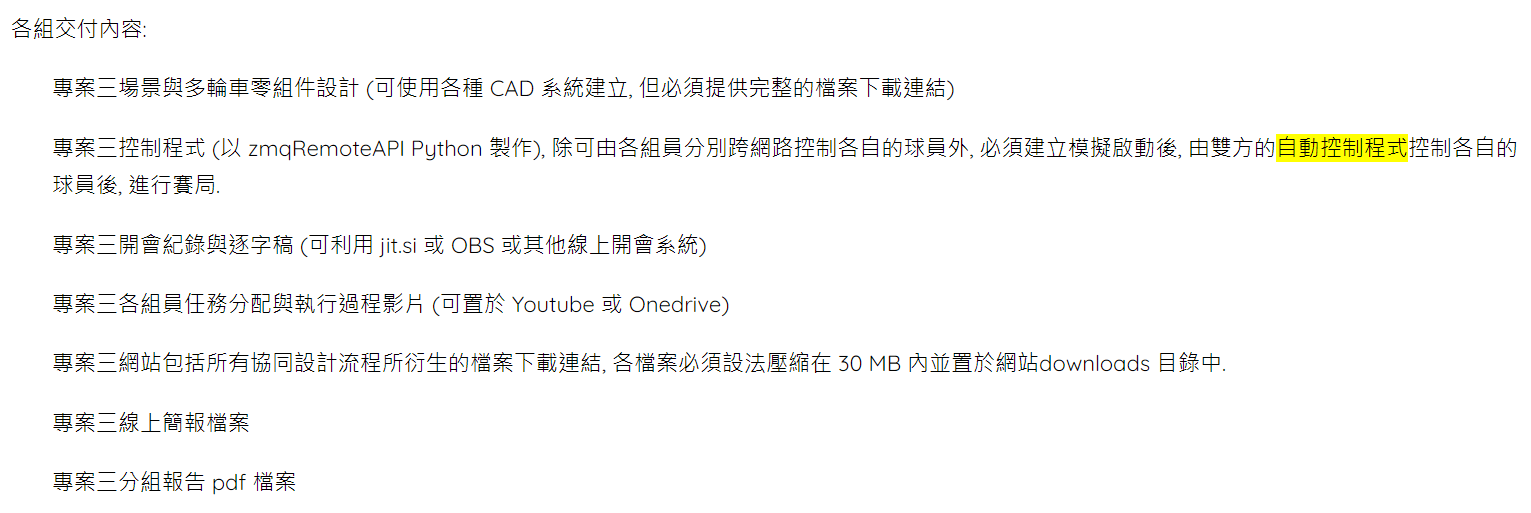
\includegraphics[height=5cm]{work}
\caption{\Large 專案目標}\label{專案目標}
\end{center}
\end{figure} 
\section{規則}
本專題設計理想為一款足球遊戲,比賽一開始球會置於場中央,遊戲開始後雙方即
可鍵盤操控機器人,透過隊友間的傳球並將球送至球門即可得分。\\
遊戲規則如下:\\
球送至敵方球門即得一分。\\
時間內進球數多的一方獲勝。\\
球進入球框後會回到原位。\\
球出界後會回到原位。\\
\renewcommand{\baselinestretch}{0.5} %設定行距
\chapter{場景建立}
\renewcommand{\baselinestretch}{10.0} %設定行距
\pagenumbering{arabic} %設定頁號阿拉伯數字
\setcounter{page}{1}  %設定頁數
\fontsize{14pt}{2.5pt}\sectionef
\section{前言}
老師有規定球場及球員的大小,重量\\
足球規格 (ball): 白色, 直徑 0.1m, 重量 0.5kg\\
足球場地 (field): 長 4m x 寬 2.5m\\
球門規格 (goal[0] and goal[1]: 長 0.6m, 高 0.3m, 寬 0.1m\\
球員尺寸範圍(player[0]-player[7]: 長寬高各 0.2m, 重量 5kg。\\
\section{建立球員}
我們使用CoppeliaSim來製作車子。\\
\

\begin{figure}[hbt!]
\begin{center}
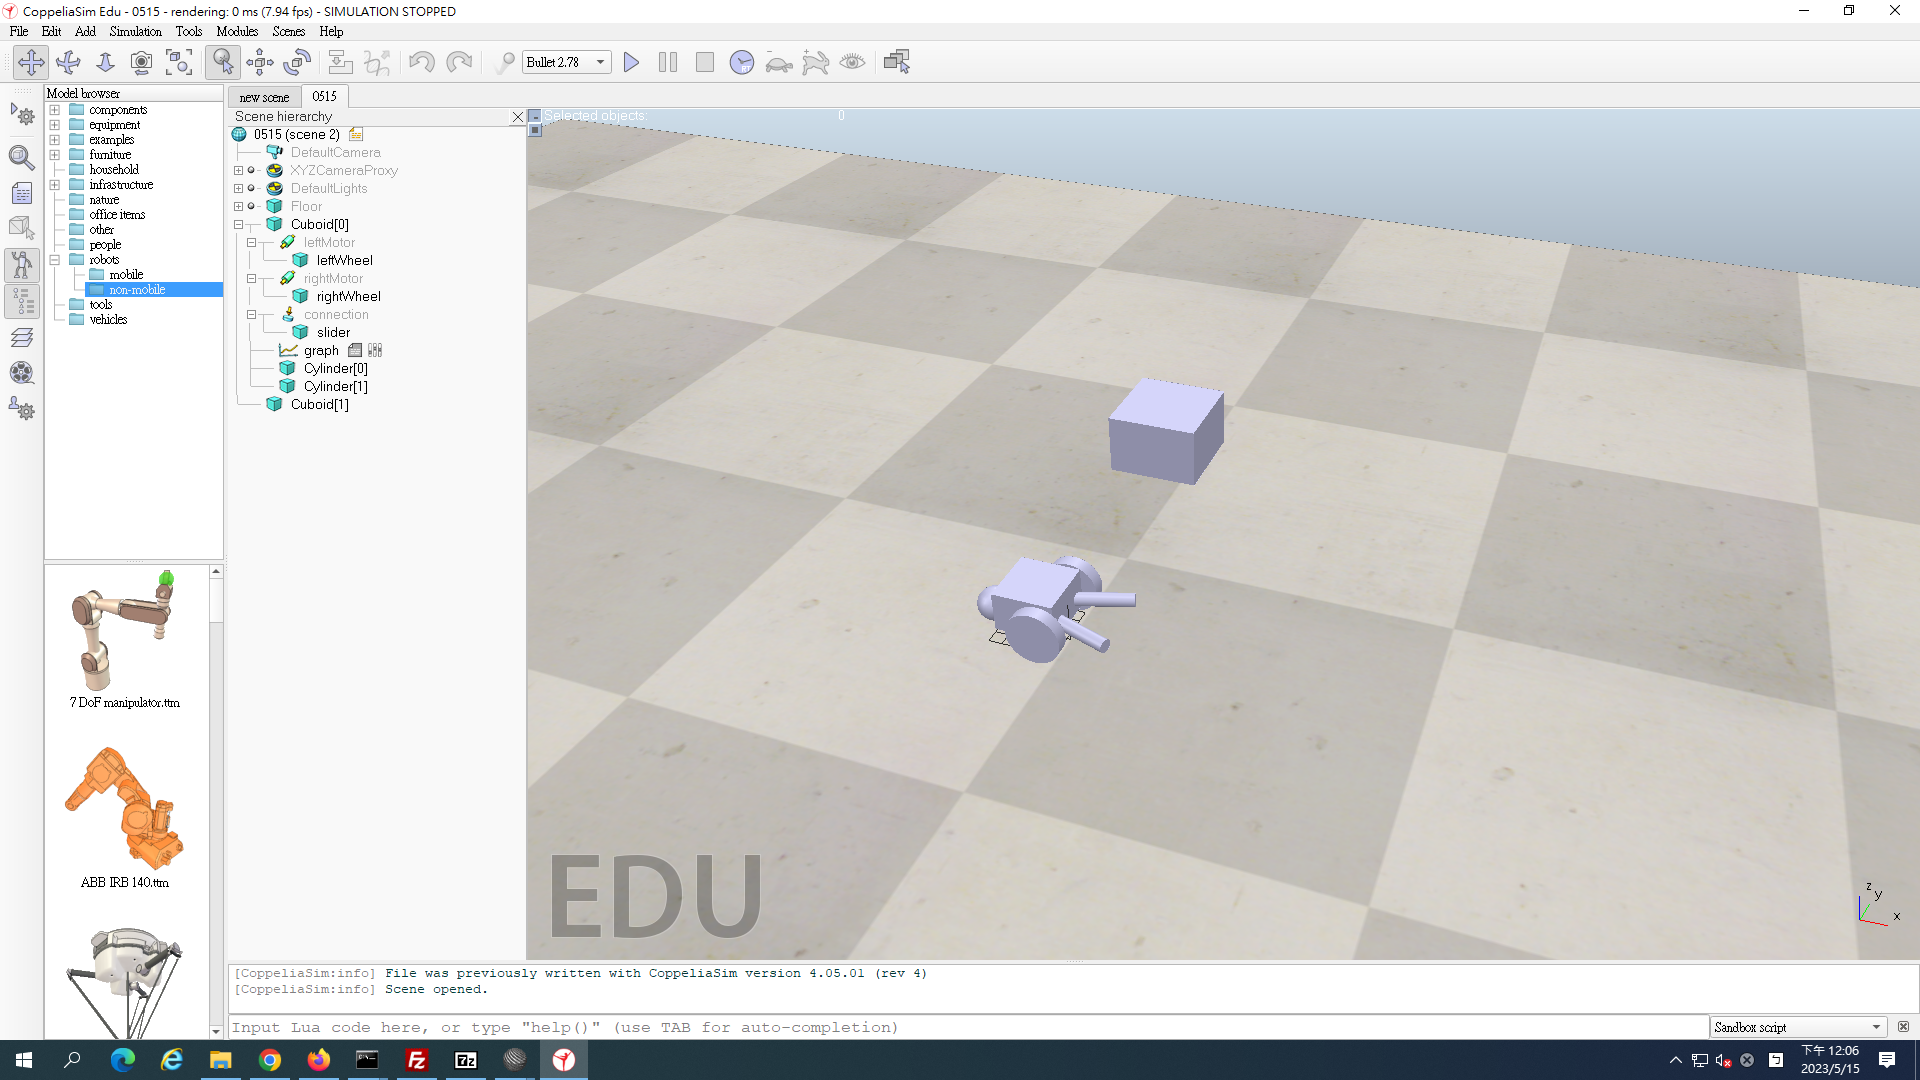
\includegraphics[width=10cm]{0515}
\caption{\Large 球員建立}\label{球員建立}
\end{center}
\end{figure}
\\
\
後發現在移動左右轉彎時會分解,因此直接在CoppeliaSim內修改了定位,且在後背加上號碼。如(圖.\ref{球員建立2})\\

\begin{figure}[hbt!]
\begin{center}
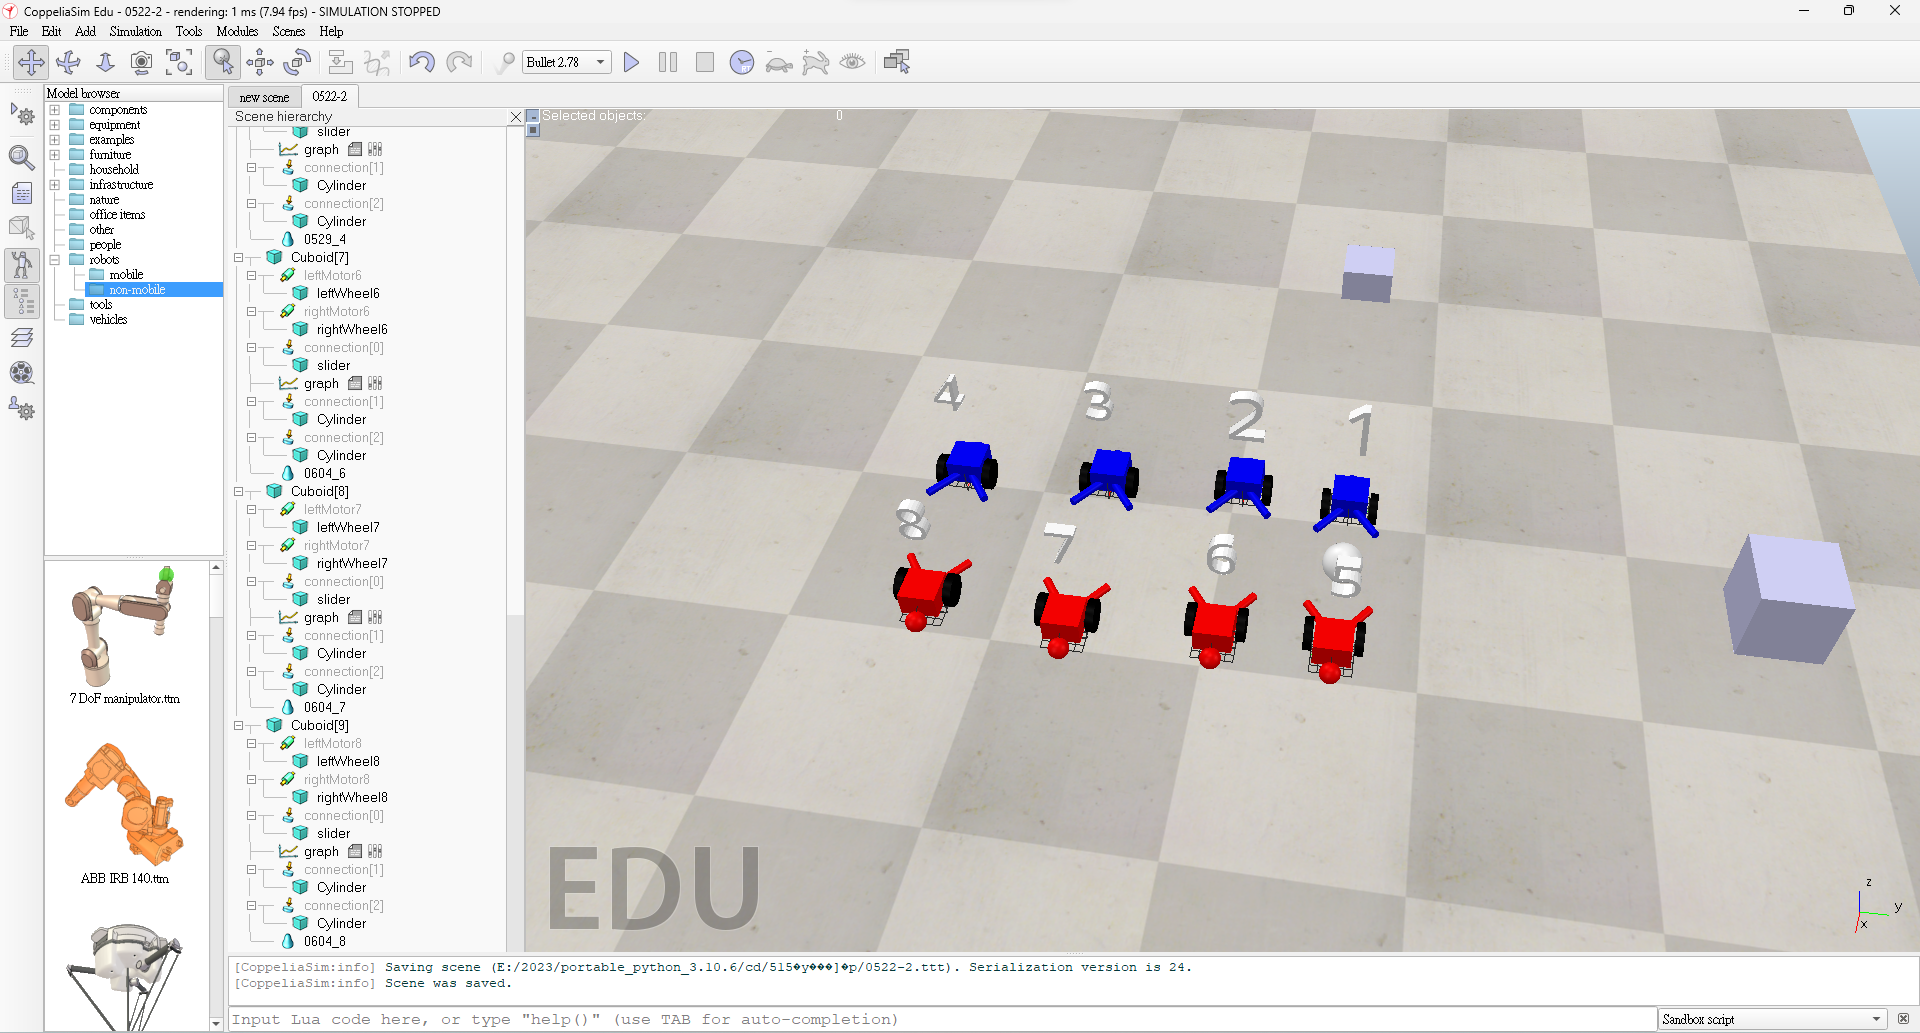
\includegraphics[width=10cm]{0604-1}
\caption{\Large 球員建立2}\label{球員建立2}
\end{center}
\end{figure}\

\section{建立記分板}
我們使用Onshape重新繪製了機械式記分板,如(圖.\ref{記分板建立})\\

\begin{figure}[hbt!]
\begin{center}
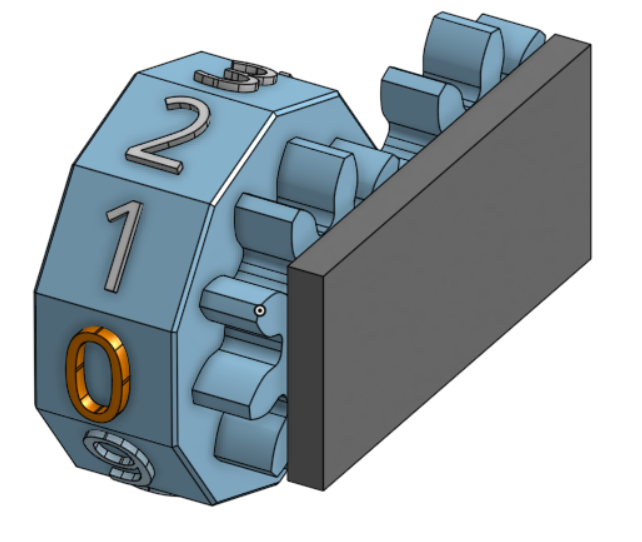
\includegraphics[width=10cm]{輪盤記分板-4-10teeth}
\caption{\Large 記分板建立}\label{記分板建立}
\end{center}
\end{figure}\

\begin{figure}[hbt!]
\begin{center}
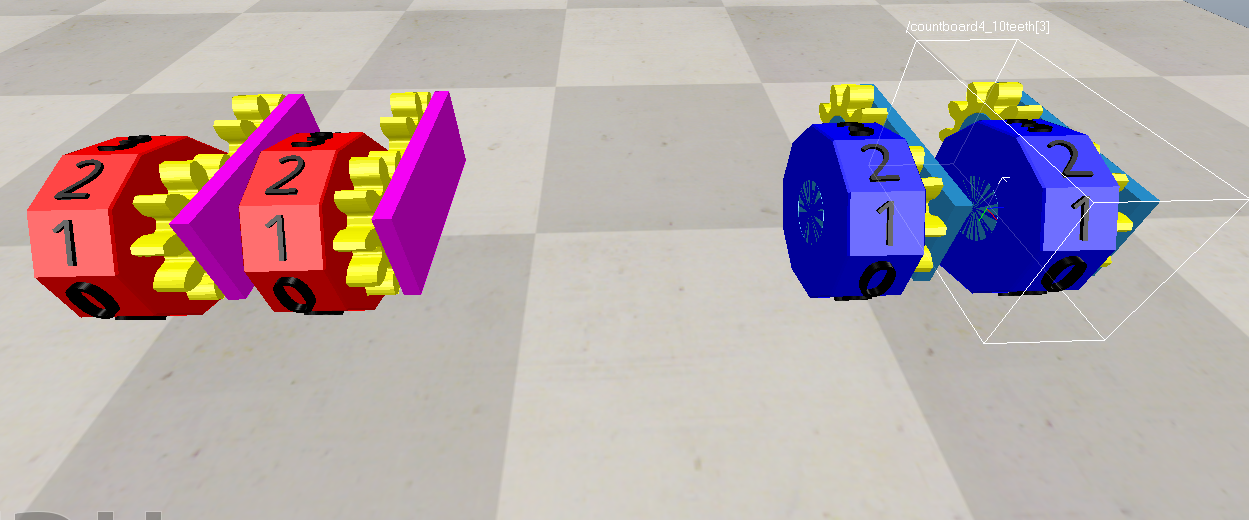
\includegraphics[width=10cm]{Screenshot 2023-05-29 113148.png4-10}
\caption{\Large 匯入記分板}\label{匯入記分板}
\end{center}
\end{figure}\
\newpage
\section{建立球場}
我們使用Onshape繪製了球場底板及球門,如(圖.\ref{球場繪製}),匯入CoppeliaSim後接著建立感測器,如(圖.\ref{建立球場})。\

\begin{figure}[hbt!]
\begin{center}
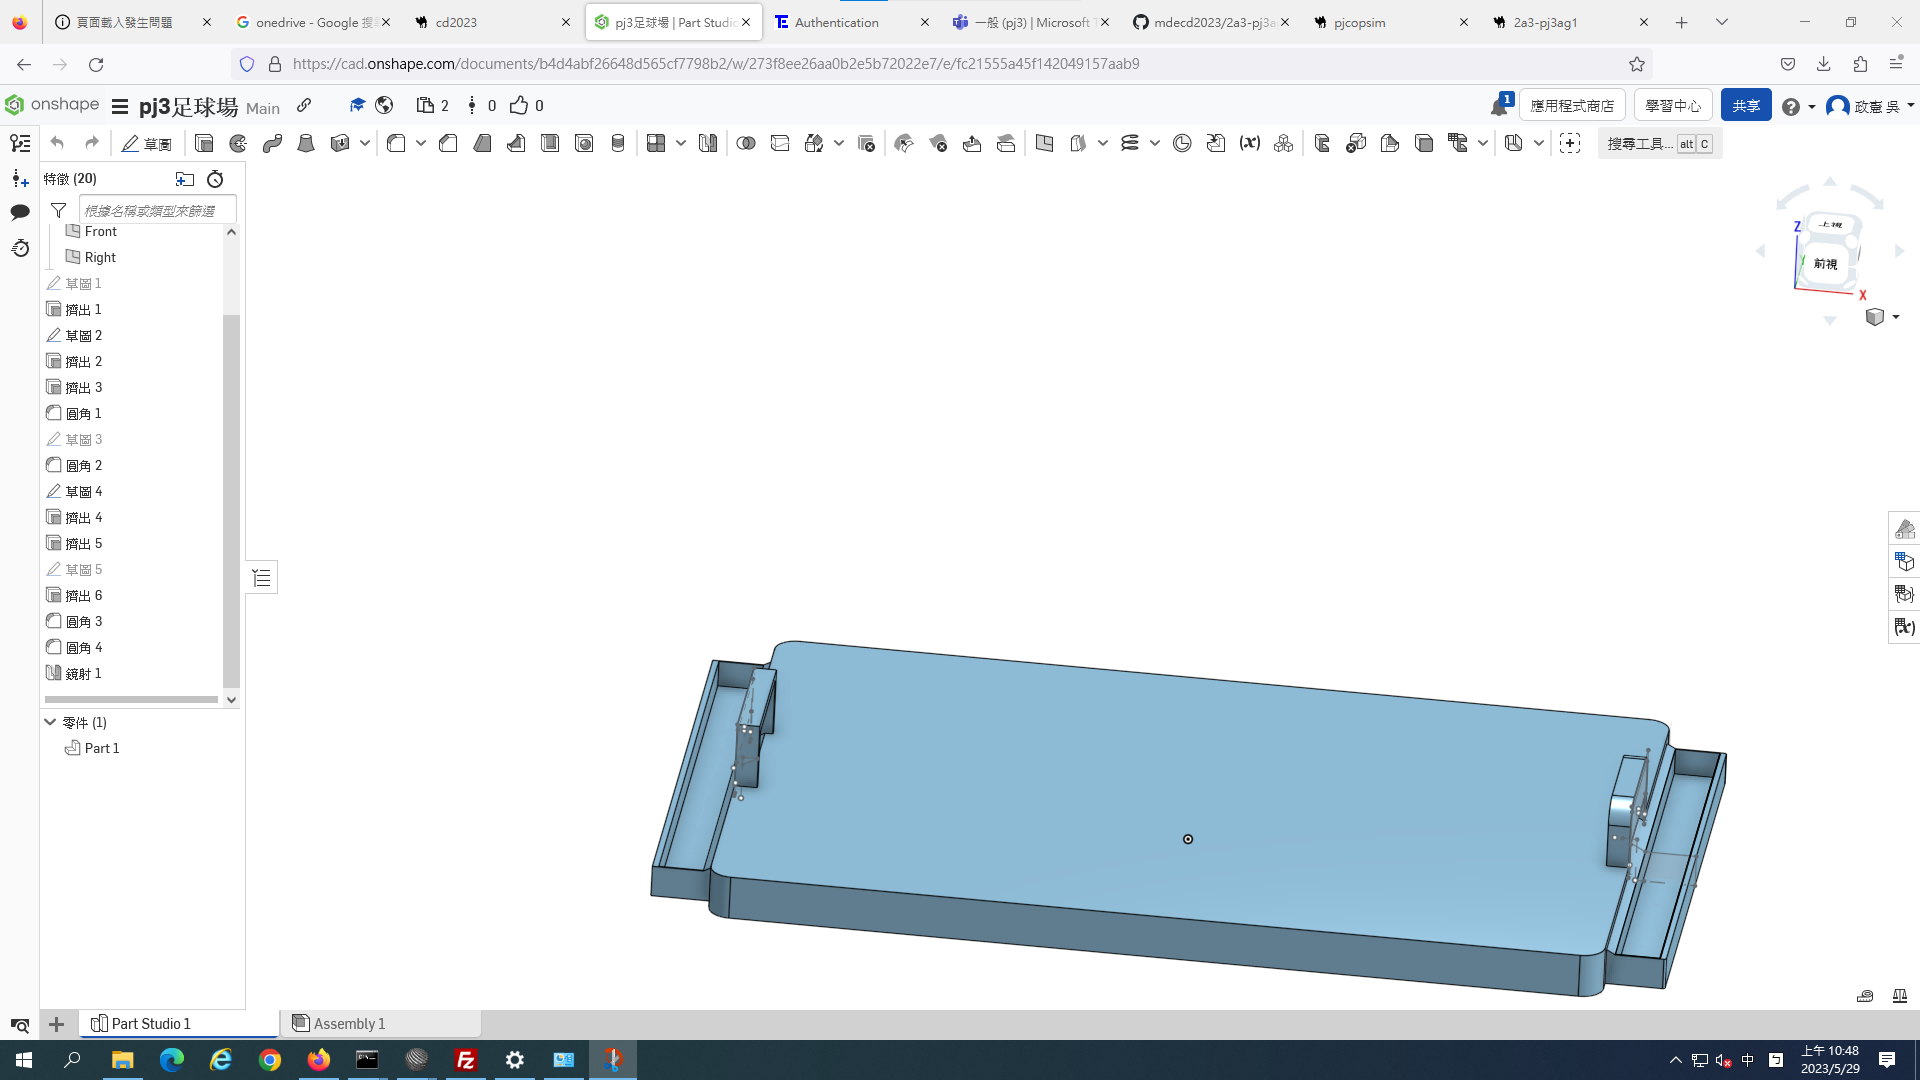
\includegraphics[width=8cm]{33333}
\caption{\Large 球場繪製}\label{球場繪製}
\end{center}
\end{figure}\


\begin{figure}[hbt!]
\begin{center}
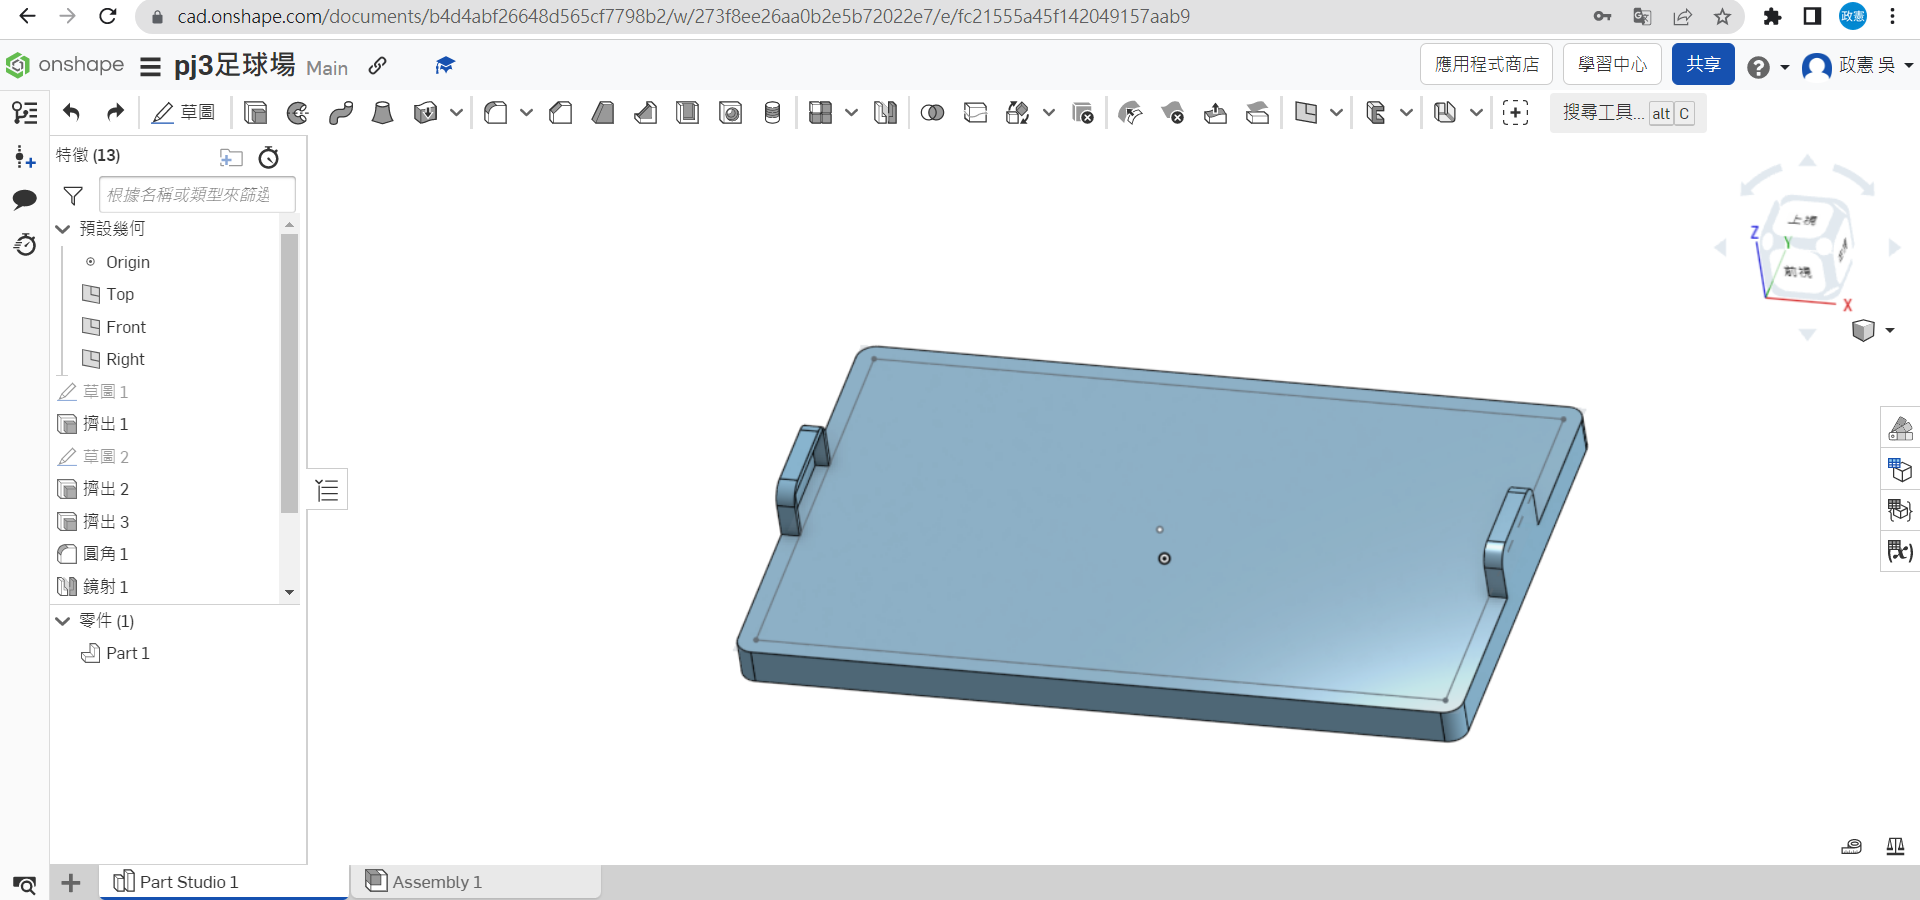
\includegraphics[width=8cm]{螢幕擷取畫面 2023-05-20 223657}
\caption{\Large 建立球場}\label{建立球場}
\end{center}
\end{figure}\

\newpage


\chapter{程式碼說明}
\renewcommand{\baselinestretch}{10.0} %設定行距
\pagenumbering{arabic} %設定頁號阿拉伯數字
\setcounter{page}{5}  %設定頁數
\fontsize{14pt}{2.5pt}\sectionef
\section{控制機器人程式}
\begin{figure}
\begin{center}
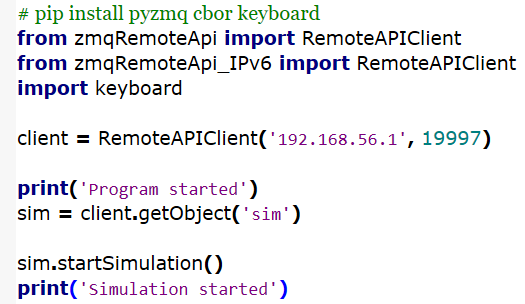
\includegraphics[height=8cm]{bubbleRob code 1}
\caption{\Large 控制機器人程式之一}\label{控制機器人程式之一}
\end{center}
\end{figure} 
使用 pip install pyzmq cbor keyboard 安裝了所需的套件,其中 pyzmq 是用於建立 ZeroMQ 連線,cbor 是用於將資料序列化和反序列化,keyboard 是用於操控鍵盤事件,使用 from zmqRemoteApi import RemoteAPIClient 和 from zmqRemoteApi_IPv6 import RemoteAPIClient 導入了用於建立與 CoppeliaSim 之間通訊的 Remote API 相關程式庫。這些程式庫提供了與 CoppeliaSim 的介面,使得可以通過程式碼控制仿真場景和物件,建立了一個 RemoteAPIClient 物件 client,並將 192.168.56.1 和 19997 分別作為 CoppeliaSim 的 IP 地址和連接埠進行初始化。這樣就建立了與 CoppeliaSim 的連線,使用 client.getObject('sim') 獲取了 CoppeliaSim 中的 sim 物件,該物件代表了整個仿真環境。透過這個物件,可以執行相關的仿真操作,再來透過  sim.startSimulation() 開始模擬。\\
\begin{figure}
\begin{center}
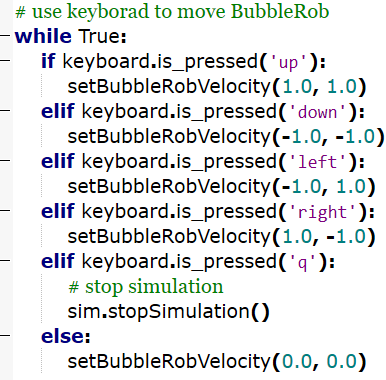
\includegraphics[height=8cm]{bubbleRob code 2}
\caption{\Large 控制機器人程式之二}\label{控制機器人程式之二}
\end{center}
\end{figure} 
這段程式碼是一個無窮迴圈,用於持續監聽鍵盤事件並根據按鍵的狀態來控制機器人的運動,如果按下 'up' 鍵,則呼叫 setBubbleRobVelocity(1.0, 1.0),將機器人的速度設定為正向。如果按下 'down' 鍵,則呼叫 setBubbleRobVelocity(-1.0, -1.0),將機器人的速度設定為反向。如果按下 'left' 鍵,則呼叫 setBubbleRobVelocity(-1.0, 1.0),將機器人的速度設定為左轉。如果按下 'right' 鍵,則呼叫 setBubbleRobVelocity(1.0, -1.0),將機器人的速度設定為右轉。如果按下 'q' 鍵,則停止仿真。若沒有按下上述任何按鍵,則呼叫 setBubbleRobVelocity(0.0, 0.0),將機器人的速度設定為零,即停止移動。
\section{模擬模型}

\newpage
\chapter{模擬環境}
%\renewcommand{\baselinestretch}{10.0} %設定行距
\section{模擬模型}
 在模擬的模型上,延用了學長設計的冰球機,並進行了部分的設計變更,將原本的人機對打更改為機器對打,且因為搭配深度強化學習的訓練,所以將兩邊的擊球器都僅保留X軸向(左右)移動,而冰球則是使用原本設計。多虧了學長們所設計的冰球機模型,讓我們在運作上有問題時可以直接發問,設計變更的地方也可以快速完成。\\
\begin{figure}[hbt!]
\center
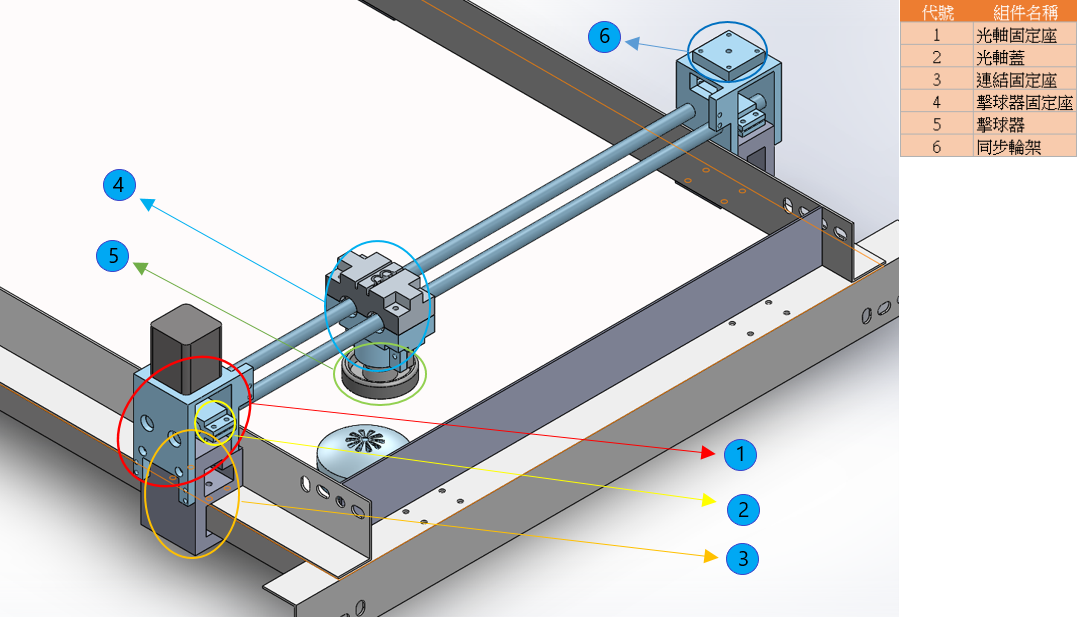
\includegraphics[width=13cm]{model}
\caption{\Large 組合圖}
\label{model}
\end{figure}

\qquad 將原本Y軸移動機構移除,並將其改為固定在特定位置上,此固定座設計是取代原本鎖在光軸固定坐上的(圖.\ref{model} 代號 1)Y軸皮帶固定座(圖.\ref{axialseat}),並使光軸固定座可以通過連結固定做鎖固於桌面,如(圖.\ref{connectSeat})。\\

\begin{figure}[hbt!]
\center
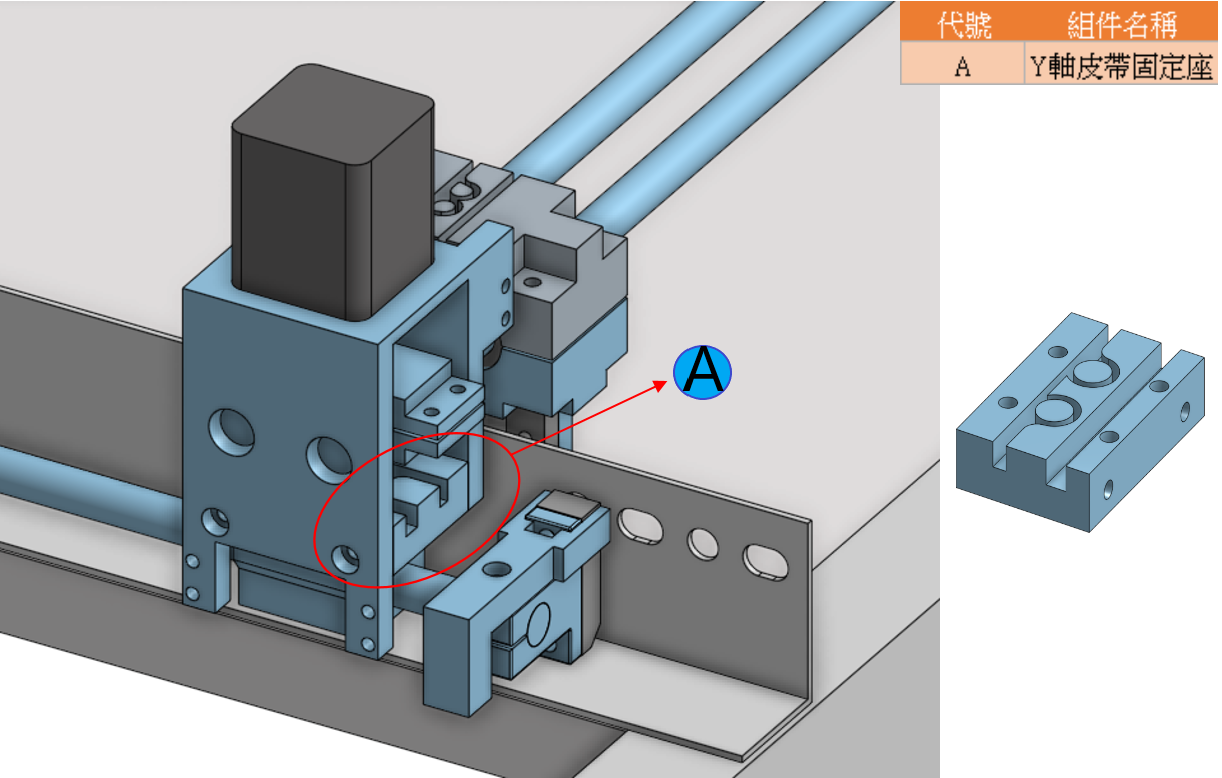
\includegraphics[width=8cm]{axialseat}
\caption{\Large Y軸皮帶固定座}
\label{axialseat}
\end{figure}

\begin{figure}[hbt!]
\center
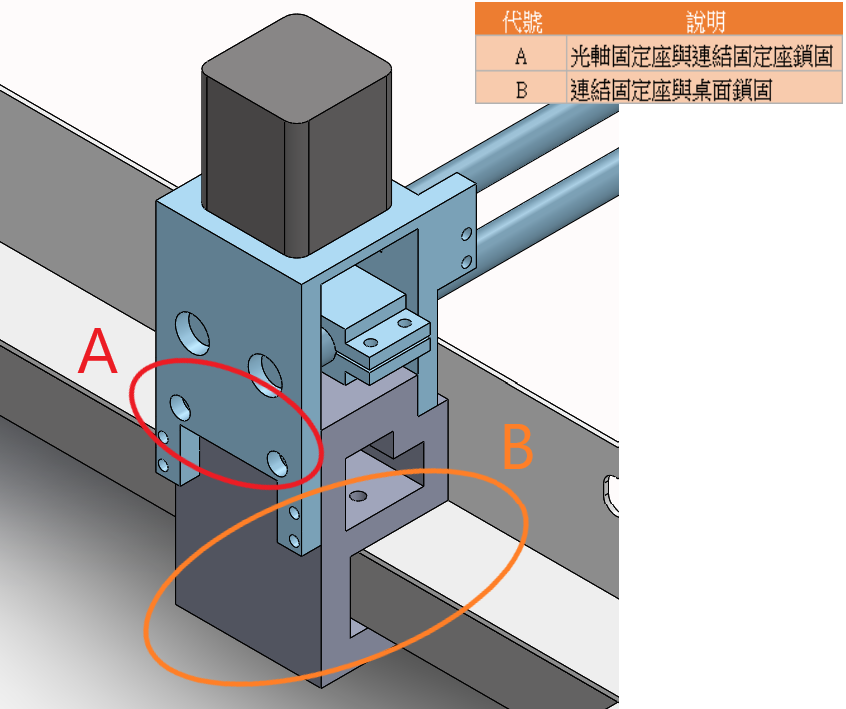
\includegraphics[width=8cm]{connectSeat}
\caption{\Large 連結固定座}
\label{connectSeat}
\end{figure}

\newpage
\qquad 分別在擊球器外側保留約冰球直徑1.5倍之區域作為得分判定區,如圖4.4中的紅色區域。\\
\section{CoppeliaSim模擬}
 CoppeliaSim是具有集成開發環境的機器人模擬器,基於分佈式控制體系架構,可以通過嵌入式腳本,插件,ROS或BlueZero節點,RemoteAPI客戶端或自定義解決方案進行模型控制。\\
 \begin{figure}[hbt!]
\center

\includegraphics[width=11cm]{CoppeliaSim}
\caption{\Large CoppeliaSim Logo}
\end{figure}

且CoppeliaSim中,控制器可以用C / C ++、Python、Java、Lua、Matlab或Octave編寫。\\
\subsection{使用原因}
 本專題之最終目標是希望可以在虛擬環境中進行深度強化學習來訓練機器對打,通過虛擬環境中的模擬後,可以更直接地看到深度強化學習訓練的狀況,且因為在虛擬環境中不會有金費的支出,所以可以不斷的重複模擬直到模擬達到最佳的狀態,除此之外CoppeliaSim的虛擬環境更接近真實環境,基於以上原因,所以使用了CoppeliaSim開發。\\
\subsection{RemoteAPI}
 RemoteAPI(Remote Application Programming Interface)是CoppeliaSim API框架的一部分。它允許CoppeliaSim與外部應用程序之間的通訊,是跨平台並支持服務調用和雙向數據流。有兩個不同的版本/框架分別為:Remote API 和The B0-based remote API。\\
\subsection{常用功能}
\begin{enumerate}
\item 以下為簡易功能說明:
\begin{figure}[hbt!]
\center
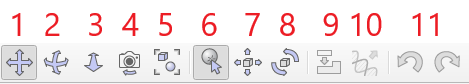
\includegraphics[width=11cm]{toolBar}
\caption{\Large CoppeliaSim 工具列}
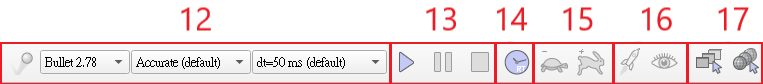
\includegraphics[width=13cm]{toolBar2}
\caption{\Large CoppeliaSim 工具列(續)}
\end{figure}
\begin{table}[hbt!]
\center
\large
\setlength{\tabcolsep}{0.75cm}{
\begin{tabular}{|c|c|c|c|}
\hline  代號 & 功能說明 & 代號 & 功能說明\\
\hline  1 &畫面平移& 10 &複製所有設定\\
\hline  2 &畫面旋轉& 11 &回復/取消回復\\
\hline  3 &畫面縮放&12&模擬設定\\
\hline  4 &畫面視角&13&開始/暫停/停止 模擬\\
\hline  5 &畫面縮放至適當大小&14&即時模擬切換\\
\hline  6 &選取物件&15&模擬速度控制\\
\hline  7 &移動物件&16&線程渲染/視覺化\\
\hline  8 &旋轉物件&17&場景/頁面 選擇\\
\hline  9 &加入/移出 樹狀結構&&\\
\hline 
\end{tabular}}
\caption{\Large 功能說明}
\end{table}
\newpage
%\item 模擬執行\\%
\end{enumerate}
\section{影像處理}

\qquad 在影像處理中我們主要使用了Python套件中的OpenCV(全稱:Open Source Computer Vision Library),並搭配其他套件或模組進行了影像處裡,藉此來取得訓練神經網路訓練時所需的資訊。\\
\begin{figure}[hbt!]
\center

\includegraphics[width=10cm]{pythonCVlogo}
\caption{\Large OpenCV 及Python logo}
\end{figure}

\subsection{CoppeliaSim中的Vision sensor(視覺傳感器)}
 CoppeliaSim的視覺傳感器輸出的影像是以每個像素中以RGB三個位元組所組成的,舉例來說:在CoppeliaSim中視覺傳感器取出畫面像素為512*256,則我們會接收到(512*256)像素*3=393,216個資料,是一筆相當大的資料,所以在影像處理上會消耗掉大量的資源。\\

\subsection{影像辨識}
 透過CoppeliaSim中的Vision sensor接收場景影像並輸出後,便可以開始進行影像辨識的處理。\\
\begin{enumerate}
\item RGB與HSV的轉換[\ref{RGBtoHSV}]\\
RGB即光的三原色Red(紅)Green(綠)Blue(藍),HSV則是一種將RGB色彩模型中的點在圓柱坐標系中的表示法,HSV分別表示Hue(色相)、Saturation(飽和度)、Value(明度),而會將RGB轉換為HSV是因為HSV相較於RGB可以更直接的判斷色彩、明暗和鮮豔度對於顏色過濾可以更方便定義出色彩範圍。\\
\begin{figure}[hbt!]
\center
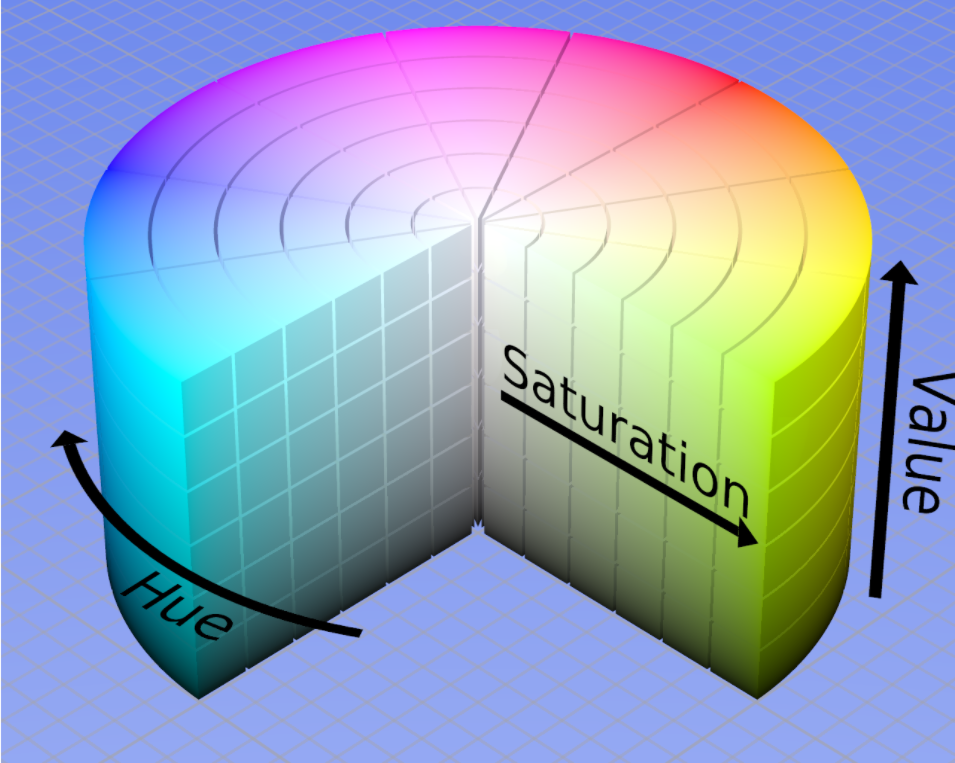
\includegraphics[width=10cm]{HSV}
\caption{\Large HSV色彩空間}
\end{figure}
\newpage
下列為RGB與HSV之間轉換的公式,首先是RGB轉為HSV,其中$max$及$min$分別為$(r,g,b)$中的最大與最小值:
$$h=\left\{\begin{matrix}
0^{\circ}, & \textrm{if}\ max=min\\ 
60^{\circ}+\frac{g-b}{max-min}+0^{\circ},& \textrm{if}\ max=r\;and\;g\geq \;b\\ 
60^{\circ}+\frac{g-b}{max-min}+360^{\circ}, & \textrm{if}\ max=r\;and\;g<  \;b\\ 
60^{\circ}+\frac{g-b}{max-min}+120^{\circ}, & \textrm{if}\ max=g\\ 
60^{\circ}+\frac{g-b}{max-min}+240^{\circ}, & \textrm{if}\ max=b
\end{matrix}\right.$$

$$s=\left\{\begin{matrix}
0, & \textrm{if}\,max=0\\ 
\frac{max-min}{max}=1-\frac{min}{max}, & \textrm{otherwise}
\end{matrix}\right.$$

$$v=max$$
接著是HSV轉為RGB:
$$\textrm{when}\,0\leq H< 360,0\leq S\leq 1,0\leq V\leq 1$$
$$C=V\times S$$
$$X=C\times (1-\left | (H/60^{\circ})\textrm{mod}2-1 \right |)$$
$$m=V-C$$

$$({R}',{G}',{B}')=\left\{\begin{matrix}
(C,X,0)& ,0^{\circ}\leq H< 60^{\circ}\\ 
 (X,C,0)& ,60^{\circ}\leq H< 120^{\circ}\\ 
 (0,C,X)& ,120^{\circ}\leq H< 180^{\circ}\\ 
 (0,X,C)& ,180^{\circ}\leq H< 240^{\circ}\\ 
 (X,0,C)& ,240^{\circ}\leq H< 300^{\circ}\\ 
 (C,0,X)& ,300^{\circ}\leq H< 360^{\circ}
\end{matrix}\right.$$


$$(R,G,B)=(({R}'+m)\times 255,({G}'+m)\times 255,({B}'+m)\times 255)$$

\item 顏色過濾\\
進行顏色過濾時,需要先定義出過濾顏色的上下限,在開始過濾後僅會保留介於上下界線範圍的影像,而介於上下限範圍之外的影像則會被剃除,如圖.\ref{filter}所示以上限(77,255,255)及下限(35,43,46)為例。\\
\begin{figure}[hbt!]
\center
\begin{minipage}[t]{0.48\textwidth}
\center
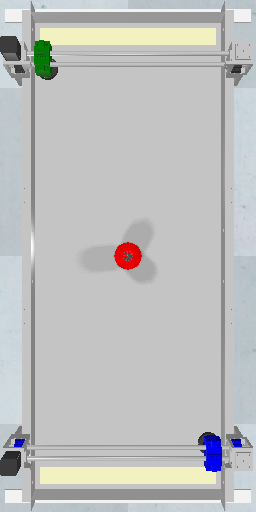
\includegraphics[width=6cm]{origin}
\caption{\Large 場景原圖}
\label{origin}
\end{minipage}
\begin{minipage}[t]{0.48\textwidth}
\center
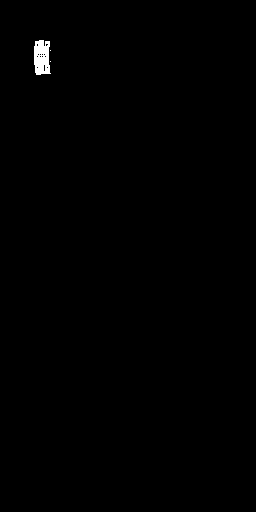
\includegraphics[width=6cm]{filter}
\caption{\Large 顏色過濾後的場景}
\label{filter}
\end{minipage}
\end{figure}


%\item 雜訊去除\\
%為了避免環境因素干擾,使影像產生雜訊並影響了影像辨識度,所以在雜訊的去除也是很重要的,

\end{enumerate}

\newpage
\chapter{伺服器}
 此專題採用 Ubuntu 20.04 版本作為我們的架設所使用作業系統,由於 Ubuntu 功能尤為繁多,以下說明重點只著重在專題製作所用到功能上。\\
 
 Ubuntu 作業系統是 Linux 系統的一個發行版,目前免費且開源,Ubuntu 基於 Debian發行版和 GNOME 桌面環境,其目標在於為一般使用者提供一個最新、穩定又主要以自由軟體建構而成的作業系統。\\
 
 其開發目的是為了使個人電腦變得簡單易用,它與其他基於 Debian 所發行的 Linux 版本更加接近 Debian 的開發理念,它主要使用自由、開源的軟體,而其他則帶很多閉源的軟體。\\
\section{Ubuntu 環境配置}
 在一開始會先使用套件管理系統 apt 指令去下載 Xorg , fluxbox , lxde 套件。Xorg 是 Ubuntu 操作系統的一個顯示服務器軟件包,它在被導入 Ubuntu 操作系統後會載入一系列的文件或軟件,這些都是跟顯示卡驅動,圖形環境庫相關的一些文件、軟件。Gnome ,kde,包括我們使用的 lxde 也需要 xorg 才能實現。而 Lxde 它的全名是 Lightweight X11 Desktop Environment ,是自由軟體桌面環境,其優點在於提供了輕量而快速的桌面環境,它比較重視實用、輕巧,除此之外它還可以在 Linux 平台執行。\\
 
 之後需選擇 display manager ( 顯示管理器 )的種類 ,Display manager 是操作系統 Ubuntu 的組件,其中登錄的動作即為 Display manager 負責。該操作系統中常見的類型有 gdm ,gdm3 , lightdm ,kdm ...。各類型的 Display manager 功能其實大同小異,差別在於外觀、操作、格式、複雜度和使用者感受等,可依使用者需求變更 ( 有些較為輕量,適合比較低階的運行器 )。選擇其中一個後繼續,之後可以切換更動 。\\

 再來是模組的導入,此處同樣用 apt 指令安裝:Pip , uwsgi , Nginx  , 以及 Git 。如果要從 Ubuntu 系統上安裝軟體,其中一種方式是 " pip "。「pip 」是 " pip Installs Packages " 的縮寫,是一個用命令列作為基礎的套件管理系統,可以用它來安裝 python 的應用程式。而使用 Git 是因為在備份資料時, 可幫助使用者有效管理原始碼,而 github 就是由 Git 伺服器和網頁介面組成,用來當作放置原始碼的倉庫。\\
 
 另外 Nginx 和 uwsgi 是為拿來配合把 python 程式應用在網路上實現,並且把想要的結果使其能在網路實時觀看操控結果之反饋。\\
\section{Oracle VM VirtualBox 介紹}
 假使建構虛擬環境時需要在同一主機使用不同電腦作業系統環境,則可使用「虛擬機器工作站」— Oracle VM VirtualBox 。\\

 選擇 Oracle VM VirtualBox    是為了因應當要使用不同作業系統 ( 比如本機與虛擬環境不同作業系統  ) 且不想與其資料存放時共用一個硬碟 ( 無多餘硬碟 , 不想硬碟之間有資料重疊 ... ) 時,即可使用其軟體做練習,降低操作失誤帶來的成本,而此軟體目前為免費,並隨時會更新,另外其特色有 :\\  
\begin{itemize}


\item 只要自備作業系統 ( 光碟片 , ISO映像檔 ) ,即可在啟動 Oracle VM VirtualBox  後直接開啟要操作的執行檔 ( 作業系統 ),不必再把主機本身重新關機,當然開啟多個作業系統之間也有共通性,可直接從視窗A做網路、檔案分享、複製貼上等動作到視窗B。\\
\item 除了作業系統裡面的執行,還可在其中練習磁碟分割、格式化以及 BIOS 啟動等 ( 但是未支援USB啟動 ) 。\\
\item 空間的佔用上並不是真實佔用空間,而是依據使用者的操作而變化 ( 使用者用多少就是多少 )。相對的,使用者雖然一開始設定該虛擬電腦的記憶體大小與硬碟空間是實時依據操作者決定,但終究還是佔掉電腦效能,所以 VirtualBox 的效能還是依據電腦本身的硬體配備。為了配置網路,首先在:
\begin{enumerate}
\item File / Preferences / Network  位置,新增一個或右鍵點擊現有的網路設定,填入該電腦網路設定 。
\item Settings / Network / Adapter 1 / Attached to: 該位置改成  Bridged Adapter
\end{enumerate}
\qquad 此處配置之比較 ( 取常用例子 ):NAT , Bridged , Internal , Host-only
\item NAT:最為基本之設定,主要讓該虛擬主機可連上網,但在與其他網路使用者互動時找不到該虛擬主機網路位址,外部網路也無法偵測,虛擬主機所有的網路請求都會把該來源視為宿主機的。
\item Host-only:虛擬主機被分配到一個網址,但是還是只有虛擬主機運行的環境可訪問該網路位址
\item Internal:此種設定主要為虛擬主機彼此間的連線,它可向外部提供資料,但反之則不行。
\item Bridged:在與其宿主機的網卡設定橋接與設定好外部網路位址後,可被外部網路訪問。
\end{itemize}
\newpage
\section{Web server}
 Nginx 是提供 web 相關服務的伺服器 ( Web server ),除了是高效能的 HTTP ( HTTPS ) 服務器外,還可處理靜態資源 , 負載平衡 , 代理等工作。代理工作為根據不同域名轉發到 Application Server 的不同 port 上去處理 ,其中又分正向和反向,正向代理為 clinet 端發送 request 經由 porxy server 再到目標網站,反向則反之。正向代理操作中 server 只知道 proxy server  給他 request , 不知道 client 是誰,而相同地反向代理則是 client 只知道 proxy server 給他 responses , 不知道 server 是誰。正向代理隐藏真實 Client,反向代理隱藏真實 Server。另外在高流量的狀況下,需要多個 Application Server 來分擔流量,負載平衡就是負責 request 的分發,決定 request 要被分到哪一個 Application Server 處理 。而關於處理靜態資源 ,Nginx 與 Apache 等 Web Server 處理靜態資源的能力是遠遠高於 Application Server 的。\\
\begin{figure}[hbt!]
\begin{center}
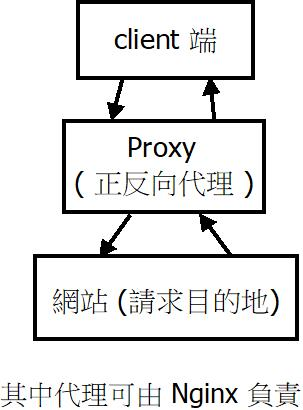
\includegraphics[scale=0.74]{clientProxy}
\caption{\Large clientProxy}\label{clientProxy}
\end{center}
\end{figure}

\section{Nginx}
\hspace{-1.7em} 網路設定:\\
 首先要修改網路設定檔,而其設定檔放在/etc/netplan目錄下的yaml檔。其中需更改的設定:
\begin{enumerate}
\item addresses:為靜態 IP,可以是IPV4或IPV6。
\item gateway:即為該電腦之閘道器。
\item nameservers:該電腦之DNS服務器。
\end{enumerate}

 WSGI(Python Web Server GateWay Interface)為一種用在Python語言上的規範,用來規範Web Server與Web Application之間如何溝通。而uWSGI同為實現了WSGI、uwsgi、http協議等的Web server,通常用於接收前端伺服器轉發的動態請求並轉發給Web Application。前者可以使用Nginx提供的https協定,且同上表述中Nginx的靜態資源處理能力較佳所以也能將靜態資源轉給其處理。\\
 
Nginx的主要設定檔nginx.conf可藉由include指令添加其他nginx設定檔的設定去擴增不同域名的設定,常見的設定有 :
\begin{enumerate}
\item 預設:
\begin{lstlisting}[caption=\Large nginx預設]
  reciveAPP {
    server localhost:5000;
    server localhost:5001;
}

server {
    listen 80;
    listen [::]:80;
    server_name SERVER_IP;
    root /home/hostname;

    location / {
            uwsgi_pass http://api/;
            include uwsgi_params;
    }
\end{lstlisting}

\newpage
\item 負載平衡LoadBalance:
\begin{lstlisting}[caption=\Large load balance設定]
  reciveAPP {
        ip_hash;
        server localhost:5000;
        server localhost:5001;
}

server {
    listen 80;
    listen [::]:80;
    server_name SERVER_IP;
    root /home/ryan;

    location / {
            uwsgi_pass 127.0.0.1:8000;
            include uwsgi_params;
    }
}
\end{lstlisting}
\end{enumerate}

 reciveAPP定義了將request proxy過去的應用,例子中server localhost語法代表可以請求proxy到分別監聽5000與5001 port的兩個應用,同時這個block可達到load balancer負載平衡的功能。\\
 
 server這個block則是定義了proxy server的相關設定,包括要監聽的port(listen 80為監聽所有IPV4位址,listen [::]80則為監聽所有IPV6位址)、規定哪些domain或ip的request會被 nginx server 處理(server\_ name)。\\
 
 location像是路由(routing)的概念,設定不同的path要對應到怎麼樣的設定。location中則是指對不同路徑的處理。\\
 
\begin{enumerate}
\item location:
\begin{lstlisting}[caption=\Large location設定]
  location / #匹配所有目錄

  location /static #匹配所有 /static 的開頭目錄
\end{lstlisting}
\end{enumerate}

 要達到load balancer透過一開始介紹的upstream block就可以達成,在上面的例子中,來自某個domain 80 port會被分配到port 5000或port 5001兩個應用中,達成用兩個應用去分擔request的負載平衡器。\\
 
 負載平衡裡的負載規則(ip\_hash )某個request要被導倒哪個應用去處理有不同規則,每個規則都有各自適合使用時機,以下簡單介紹幾個常見的規則:\\

\begin{enumerate}
\item round-robin(預設)輪詢方式:也就是將請求輪流按照順序分配給每一個 server。假設所有伺服器的處理效能都相同,不關心每臺伺服器的當前連線數和響應速度。適合於伺服器組中的所有伺服器都有相同的軟硬體配置並且平均伺服器請求相對均衡的情況。
不過也有另外一種可以設定權重的Weight Round Robin(加權輪詢方式),可以設定不同server的權重,例如以下範例:
\begin{lstlisting}[caption=\Large 設定不同 server 的權重]
  upstream myweb {
    server web1.dtask.idv.tw weight=3;
    server web2.dtask.idv.tw weight=2;
}
\end{lstlisting}
\item least-connected 最少連線:顧名思義為連線進來時會把Request導向連線數較少的Server。
\item IP-hash依據Client IP來分配到不同台Server:通過一個雜湊(Hash)函式將一個 IP 地址對映到一臺伺服器。先根據請求的目標IP地址,作為雜湊鍵(Hash Key)從靜態分配的散列表找出對應的伺服器。除非斷線或IP變動,否則同個IP的請求都會導入到同一個 server。
\end{enumerate}
  uWSGI設定(uwsgi\_ini ):
 \begin{enumerate} 
 \item wsgi-file:主要運行的py檔案
 \item http,socket,http-socket:端口設定,假使有使用到 前端服務器(如Nginx)時,不能用http設定,因uwsgi協議為HTTP,而Nginx使用傳輸協議為TCP,兩者不能互通。
 \begin{lstlisting}[caption=\Large 簡易uwsgi指令啟動]
  uwsgi --http:9000 --wsgi-file APP.py 
\end{lstlisting}
 \item processes、threads:工作序,processes為進程,threads為線程,下方設定為每條近程有兩條線程。
 \begin{lstlisting}[caption=\Large 加入工作程序uwsgi指令啟動]
  uwsgi --http:9000 --wsgi-file APP.py --processes 4 --threads 2
\end{lstlisting}
\item chdir:此項是為了正確的加載模組/檔案 \\
整體快速配置(這裡儲存成一個.ini文件,其他還有YAML、JSON、XML格式等):
\begin{lstlisting}[caption=\Large 將uwsgi指令啟動動作設定成一個啟動檔]
  [uwsgi]
socket = :9000
processes = 4
threads = 2
chdir = location/to
wsgi-file = location/to/file
\end{lstlisting}
此項還可加上status:此項為查看uWSGI內部的輸出數據\\
\begin{lstlisting}[caption=\Large status]
  -- status 127.0.0.1:9001
\end{lstlisting}
實現之通訊流程 

\begin{figure}[hbt!]
\begin{center}
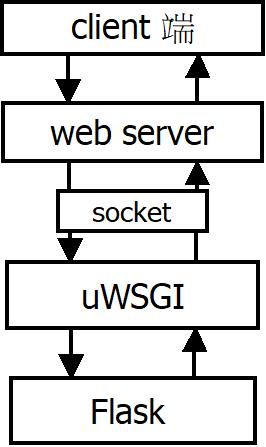
\includegraphics[scale=0.74]{clientToflask}
\caption{\Large client To flask}\label{clientToflask}
\end{center}
\end{figure}
 \end{enumerate}
\section{Flask}
 
 如同以上所述,建立Flask框架的同時需選擇反向代理伺服器(這裡我們選擇了Nginx)來負責網頁請求和結果的回覆,同時還需要一個實現WSGI通信協議的伺服器(我們選擇了 uWSGI)來負責接收代理伺服器的請求後Flask轉發及接收訊息,再轉發回去(代理伺服器)。\\
 
\begin{figure}[hbt!]
\begin{center}
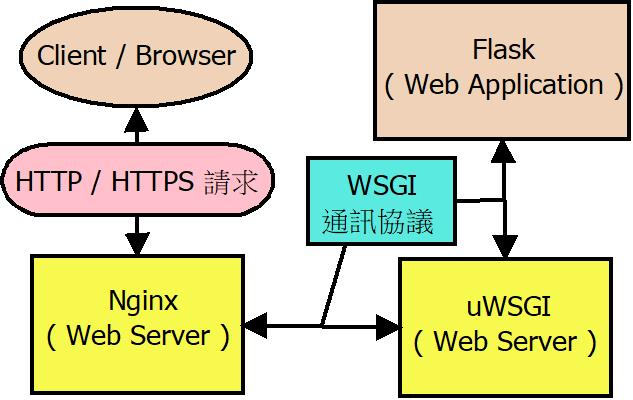
\includegraphics[scale=0.74]{total}
\caption{\Large total}\label{total}
\end{center}
\end{figure}

\chapter{機器學習的訓練與模擬控制結果}
\section{訓練模型的基礎概念}
 訓練模型的原型是實體冰球機的機電系統,由於要訓練強化學習,所以需要將模型簡化至最簡潔的方式進行訓練,並取Open AI Gym的環境當作最簡化的訓練模型。由於強化學習是一種最佳化控制的方式,因此將Gym的Pong畫面當作輸入,輸出為擊錘移動方向,藉由調整當中的權重、偏差等參數,將參數調配到最優狀態。將可行的訓練方式套用到CoppeliaSim進行虛擬環境的訓練,並且可將訓練結果套用到實機進行運用。\\
\section{訓練模型的選用}
 利用Gym的環境訓練機器學習,以測試學習率、神經網路隱藏層的神經元個數、機器學習的啟動函數類型、訓練時影像大小等幾項參數與訓結果之間的關聯性,選用pyhton語言進行配置。剛開始我們運用Pygame模組來撰寫pong game的訓練環境,開始學習並了解Pygame的一些運用,嘗試建構出pong game場景(圖.\ref{fig.pong_pygame}),在基本功能編寫告一段落後,測試程式漏洞,發現對打時特定角度碰撞,球會超過擊錘的碰撞感測,導致出現球擊穿擊錘的現象。為了解決Pygame碰撞問題,做了幾種嘗試:修改Pygame的碰撞定義,更換碰撞感測的感測方式,問題依舊沒有顯著的改善,若增加過多的碰撞偵測點則會造成後續機器學習訓練時的運算負荷;另一種方法則是搭配pymunk的物理引擎模組使用(圖.\ref{fig.airhockey_pymunk}),使環境更符合實際物理現象,可加入碰撞、摩擦、力量大小、速度大小等可以個別設定和調用。當環境有了物理接下來就需要加入訓練所需的功能,如:訓練時的場景的即時影像畫面、即時獎勵回傳、該局結束時的場景重設和分數重置等功能。此時找到了Open AI Gym模組。\\
\begin{figure}[hbt!]
\begin{center}
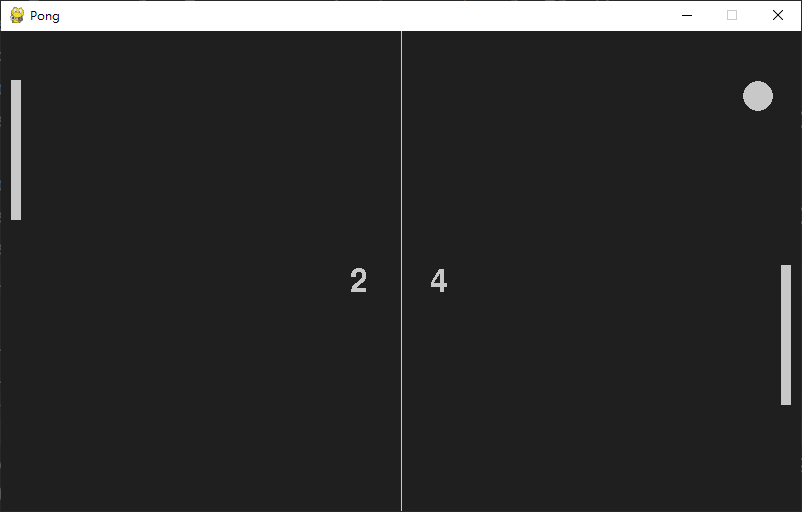
\includegraphics[width=12cm]{pong_pygame}
\caption{\Large Pygame模組編寫}
\label{fig.pong_pygame}
\end{center}
\end{figure}

\begin{figure}[hbt!]
\begin{center}
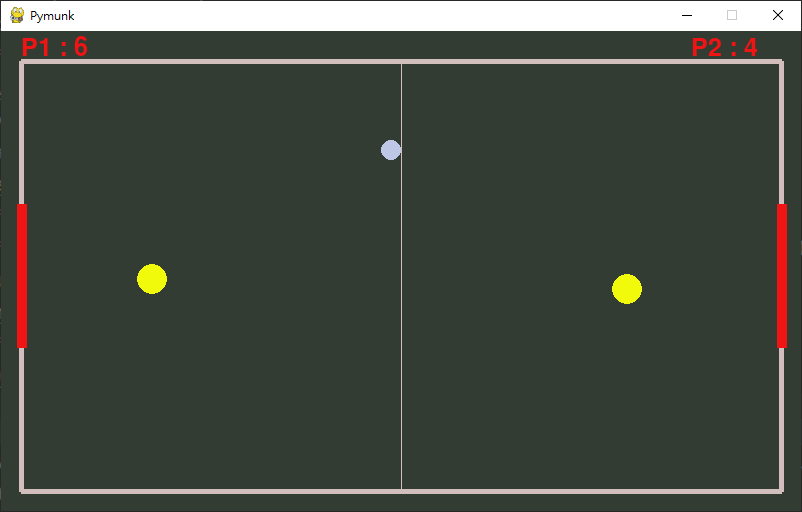
\includegraphics[width=12cm]{airhockey_pymunk}
\caption{\Large Pymunk模組編寫}
\label{fig.airhockey_pymunk}
\end{center}
\end{figure}
 \newpage %圖片空隙勿刪
 Open AI Gym裡面有十幾種訓練模型的環境,提供機器學習做訓練的環境。由於我們的訓練模型是pong game,在Gym模組裡面剛好有訓練模型,因此使用Gym模組相對於使用Pygame和pymunk的搭配來的方便,而且後續要在CoppeliaSim模擬環境模擬時也有套件可搭配使用,可簡化功能和訓練時所需的環境模型和訓練功能的程式編寫,另一方面自寫場景需要測試場景的漏洞,使用Gym可以節省檢查場景漏洞和修正的時間。\\
\section{訓練程式的運作}
 由於機器學習和影像處理需要大量的運算矩陣運算,因此如果只單獨透過Python本身運算比編譯語言執行的速度來的慢,所以使用Numpy程式庫來解決在Python環境矩陣運算速度慢的問題,以提升訓練機器學習時的運算效率。pickle是Python內部的序列化方式,主要是當機器學習訓練時可能因為一些原因需要暫時停止訓練,但為了讓已經停下的訓練再次重啟就需要透過pickle序列化的方式,將暫停前的訓練權重值透過pickle將其記錄下來,當訓練再次重啟時就可透過pickle.load讀取先前紀錄的pickle檔案就可回到當時暫停的狀態下繼續進行訓練。\\
 
 機器學習所運用的架構是強化學習並搭配神經網路來訓練機器學習,結合了強化學習不需要事先收集訓練資料、不需要特別教導,以及神經網路的非線性激活函數的計算和參數的記憶性。\\

\begin{figure}[hbt!]
\begin{center}
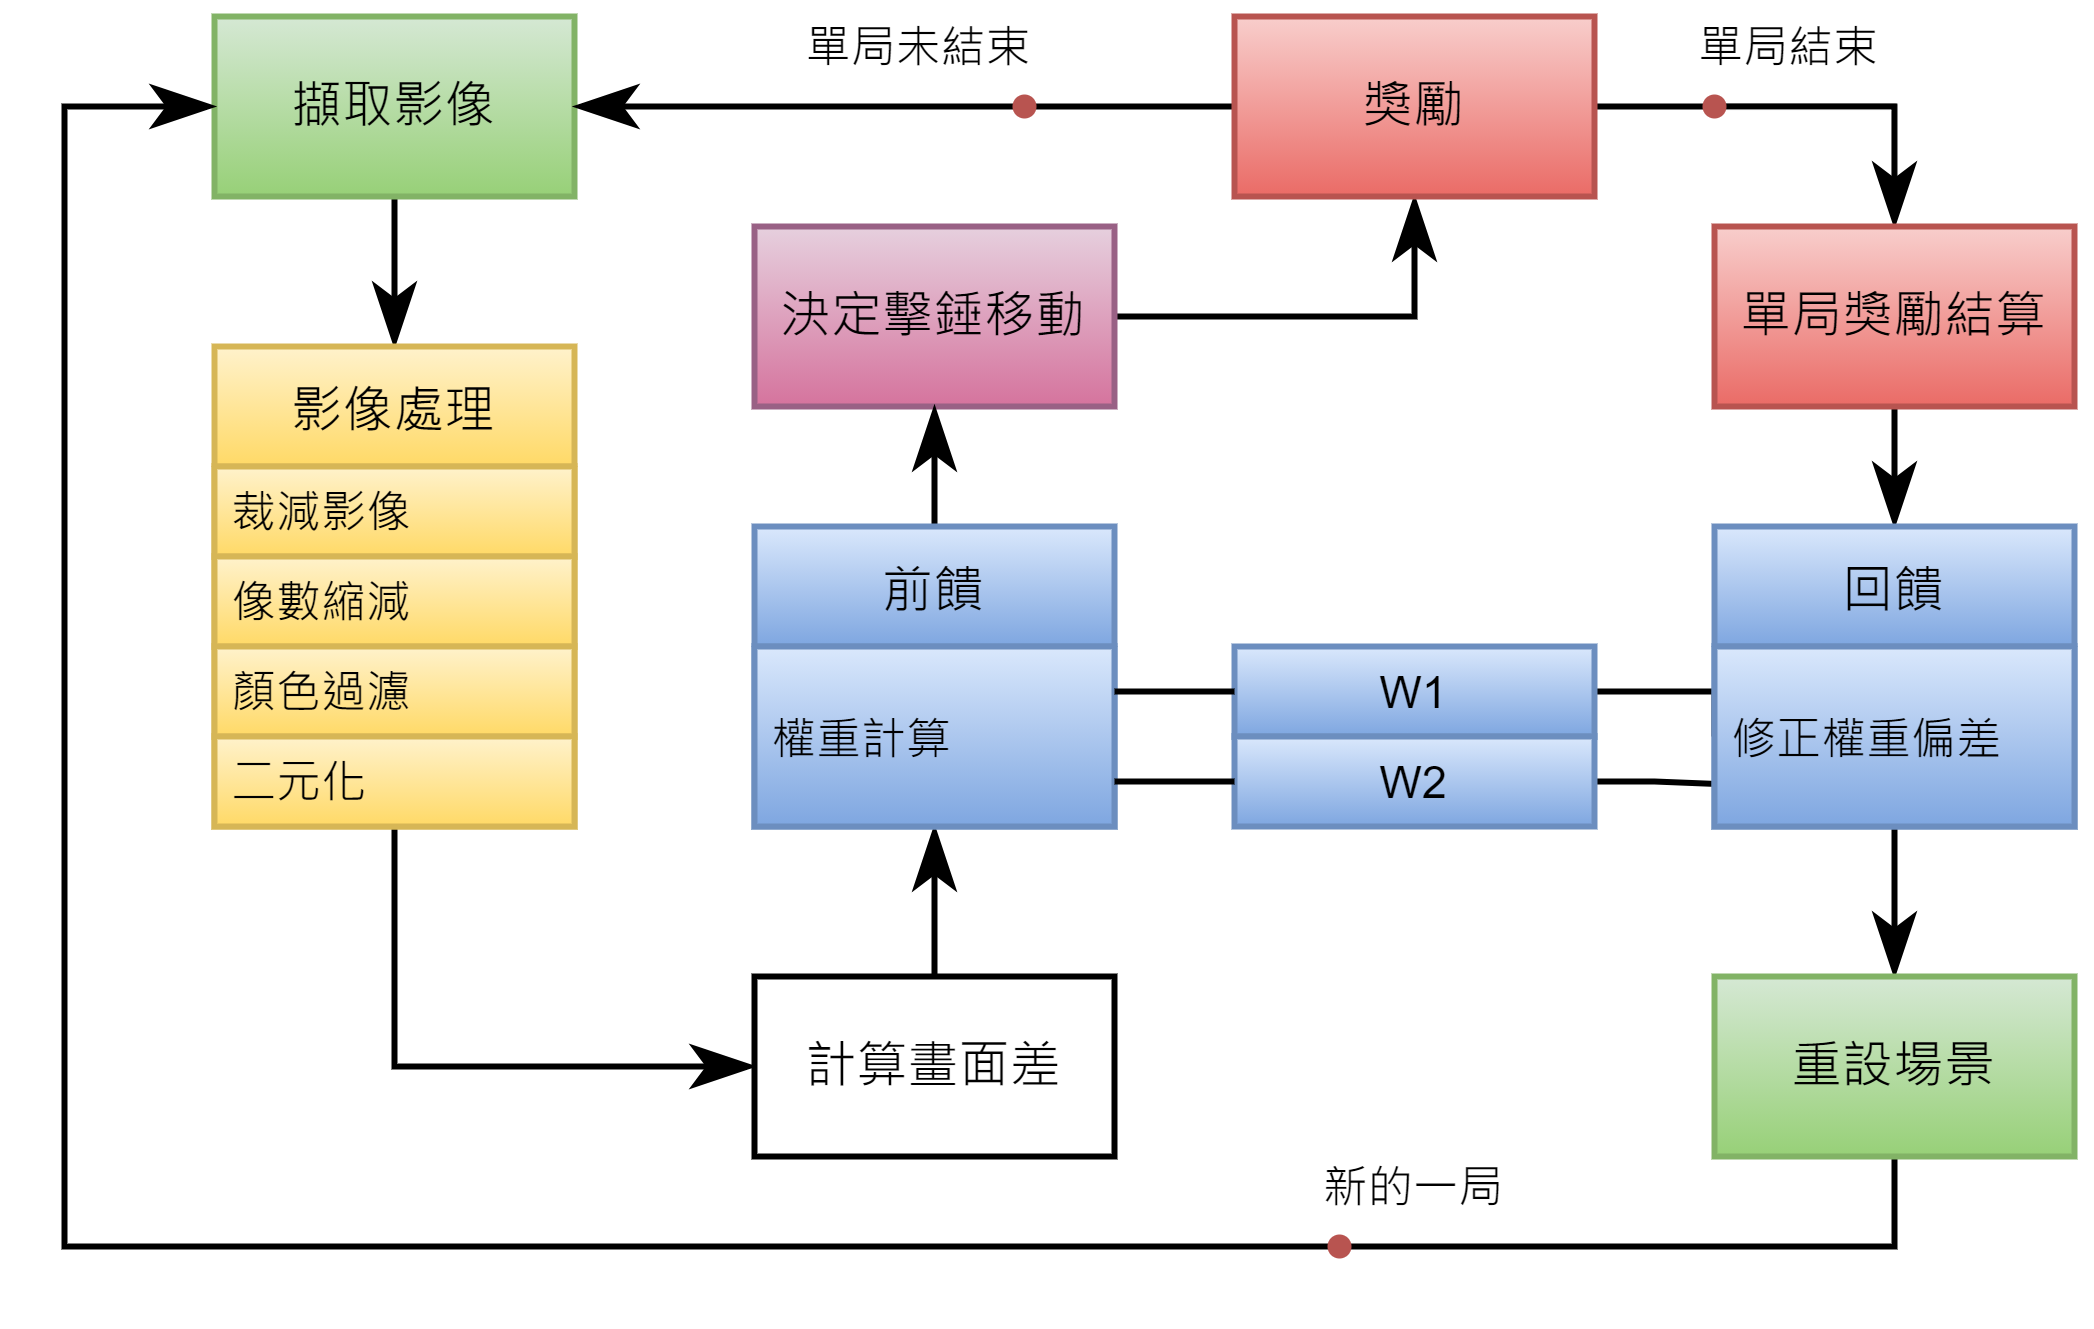
\includegraphics[width=15cm]{強化學習訓練流程}
\caption{\Large 強化學習訓練流程}
\label{fig.強化學習程式流程}
\end{center}
\end{figure}
%-----------------------------%

%=---------圖片空隙勿刪--------=%
%-----------------------------%
程式訓練流程(圖.\ref{fig.強化學習程式流程}):\\
 擷取影像,將影像裁剪至實際遊戲範圍,並簡化像素以利提高訓練時的計算速度,減少運算時的負擔,過濾顏色只保留球與擊錘,並把取到的影像二元化,取兩幀畫面進行比較,掌握球與擊錘間的相對位置(畫面差),透過前饋:計算球在環境的狀態及擊錘移動的決策,畫面差透過W1權重來計算球在環境的狀態,透過W2權重並經過啟動函數(activation function)得出擊錘移動的決策。透過產生隨機值的方式來與擊錘移動決策值進行比較,判定隨機值落在的區間來決定移動策略。計算discount reward及獎勵的加總。獎勵設定球若超過了對手,獎勵為+1;如果錯過球,則獎勵為-1;其餘狀態獎勵為0。\\

 在單局結束時,紀錄下該局累積下來的經驗,亦是紀錄該局所修正出來的參數而進行獎勵計算、log probability、RMSprop優化率減因子和反饋(back propagation),當訓練次數到達指定次數會以pickle做紀錄,存下的數據可再次導入模型進行實際運用,或是當程式中斷後可重新匯入進行訓練。比較持續訓練與中斷後重新匯入訓練的差異,測試算法版本為Pong2,MSE代表均方誤差值,pong2\_ r表示中斷後重新匯入的訓練數據,pong2與pong2\_ r標示個別表示該訓練每局分數的紀錄,pong2 MSE與pong2\_ r MSE標示個別表示該訓練均方誤差值紀錄(圖.\ref{fig.比較中斷數據}) \\
\begin{figure}[hbt!]
\begin{center}
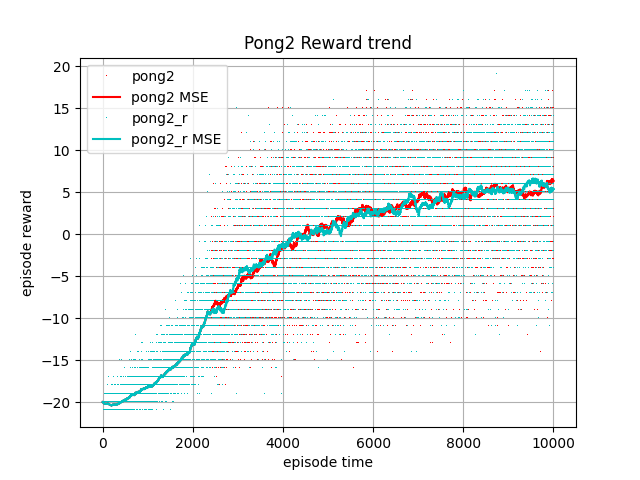
\includegraphics[width=15cm]{pong2_RvsNR}
\caption{\Large 比較中斷後訓練差異}
\label{fig.比較中斷數據}
\end{center}
\end{figure}

\section{訓練算法與參數比較}
 pong1版本是karpathy的pg\- pong.py的原始碼[\ref{R.pong1}],pong1.1原始碼則是schinger的pong\_ actor\- critic/pg\- pong\- ac.py[\ref{R.pong1.1}],pong1.2的是修改pong1的學習率參數從0.001調整到0.0001,並且將裁切後80*80的影像改成75*80。pong2版本是etienne87的pg\- pong.py的原始碼[\ref{R.pong2}]修改的,將動作策略由上下上替換成停上下的模式,學習率也配合調整,由0.0001調至0.001。\\
 
 下圖(圖.\ref{fig.比較中斷數據})為這幾個版本的訓練趨勢的紀錄提供做比較,訓練次數(圖.\ref{fig.比較中斷數據}之水平軸)為3000局做比較,小點為每局積分總和(圖.\ref{fig.比較中斷數據}之垂直軸),線條為累積積分的均方誤差值,積分計算$-21$分代表對面得21分,即機器訓練所得分數-對面所得分數。訓練存在隨機性(Stochastic),因此每次訓練所得趨勢會有所差異。\\
\begin{table}[hbt!]
\center\large
\setlength{\tabcolsep}{0.75cm}{
\begin{tabular}{|c|c|c|c|}
\hline  版本名稱 & 標示顏色 & 啟動函數 & 參考來源\\
\hline  pong1 &  紅色 & sigmoid & [\ref{R.pong1}]\\
\hline  pong1.1 &  藍色 & sigmoid & [\ref{R.pong1.1}]\\
\hline  pong1.2 &  橘色 & sigmoid & [\ref{R.pong1}]\\
\hline  pong2 & 綠色 & softmax & [\ref{R.pong2}] \\
\hline
\end{tabular}}
\caption{\Large 版本標示}
\end{table}

\begin{figure}[hbt!]
\begin{center}
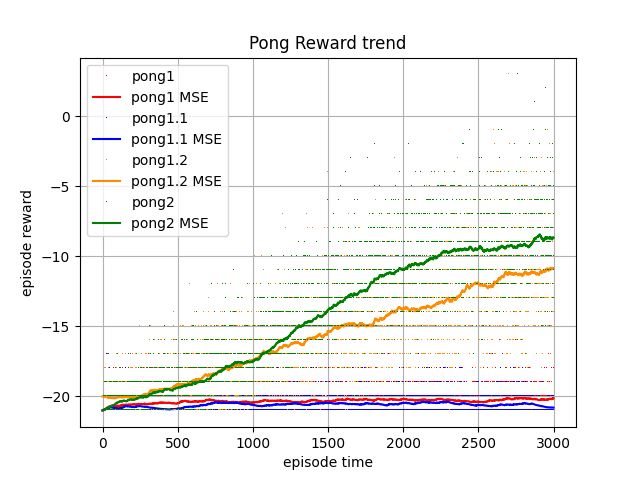
\includegraphics[width=15cm]{pong}
\caption{\Large 各版本差異}
\label{fig.各版本差異}
\end{center}
\end{figure}
觀察後發現,pong2版本的訓練結果得分最高,pong1.2的訓練結果為次高,pong1及pong1.1的版本沒有收斂,訓練對打的表現沒有進步的跡象,參數還需做調整及測試,pong2及pong1.2為主要選擇訓練演算法。接下來測試pong1的學習率調整成0.0001,pong1.2的學習率上調到0.001,以pong2版本當作對照(圖.\ref{fig.比較中斷數據}),同樣以3000次訓練當作參考依據,測試結果三者相當接近。因為訓練時間及設備限制,修正後的pong1與pong1.2版本所以擇一與pong2進行長時間訓練比較,因此選用pong1.2版本。

\begin{figure}[hbt!]
\begin{center}
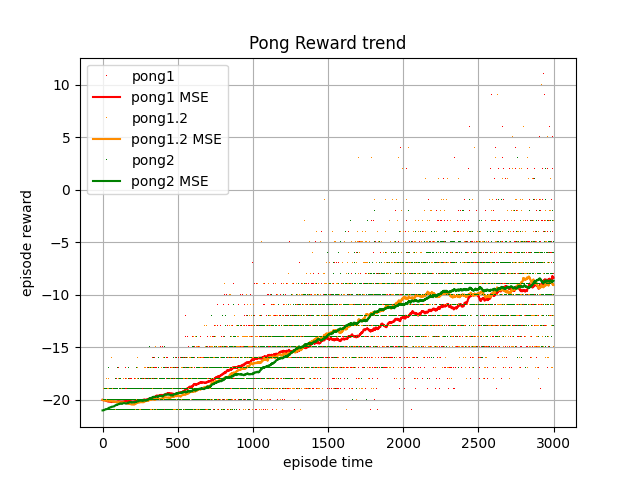
\includegraphics[width=15cm]{pong_test}
\caption{\Large pong1與1.2調整後數據比較}
\label{fig.調整後數據比較}
\end{center}
\end{figure}

\begin{flushleft}
電腦規格:\\
\end{flushleft}
\begin{enumerate}[1.]
\item 研究室桌上型電腦(長時間訓練所使用):\\
Windows10 專業版 2004\\
CPU:Intel i7-7700 3.60GHZ\\
RAM:16GB\\
GPU:NVDIA GTX1050
\item 個人筆記型電腦(3000次訓練數據為此設備訓練,短時間測試用):
Windows10 家用版 2004\\
CPU:Intel i7-8750H 2.20GHZ\\
RAM:8GB\\
GPU:NVDIA GTX1050 Ti\\

總訓練時數約336\textasciitilde 350小時(圖.\ref{fig.pong2與pong1.2長時間訓練比較}),pong2的數據均方誤差(MSE)數據較穩定,由於訓練中無法得知當下是處於數據波動的較優或較差的狀態,若要中斷訓練則有可能剛好處於波動的較差的狀態,因此選擇pong2的版本當作訓練算法較為穩定。
\end{enumerate}
\begin{figure}[hbt!]
\begin{center}
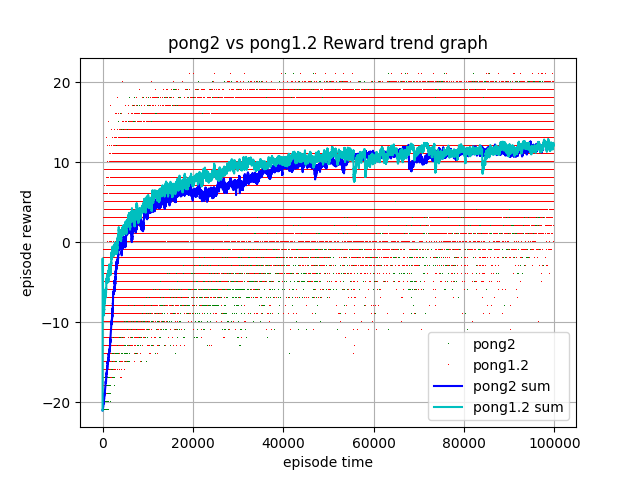
\includegraphics[width=15cm]{pong2_vs_pong1.2_reward}
\caption{\Large pong2與pong1.2長時間訓練數據}
\label{fig.pong2與pong1.2長時間訓練比較}
\end{center}
\end{figure}



\section{CoppeliaSim RemoteAPI}
在進行強化學習時主要是透過CoppeliaSim中的Remote API 函數來取得模擬場景中所需要的資訊,並在進行訓練後再回傳到CoppeloaSim做控制的動作。\\
\subsection{Remote API模組及動態連結函示庫}
在啟用RemoteAPI需要先準備以下三項模組和動態連結函示庫,並將此三項與預執行的程式放在同一目錄下:
\begin{itemize}
\item sim.py
\item simConst.py
\item remoteApi.dll、remoteApi.dylib 或 remoteApi.so (依序適用於:Windows、MacOS、Ubuntu)
\end{itemize}
sim.py及simConst.py為Python模組,其位於:\\
CoppeliaSim安裝目錄$\backslash$programming$\backslash$remoteApiBindings$\backslash$python$\backslash$python\\
remoteApi.dll為RemoteAPI動態連結函示庫,其位於:\\
CoppeliaSim安裝目錄$\backslash$programming$\backslash$remoteApiBindings$\backslash$lib$\backslash$lib$\backslash$作業系統\\
\subsection{Remote API埠使用}
Remote API是通過通訊埠取得環境資訊,在CoppeliaSim中預設埠號為19997,只有預設埠不需開啟特定場景就可進行通訊並控制所有功能,且在大量影像資料處理時可啟用多埠,使其中一個通訊埠用於影像處理,另一個則用於控制,新增的通訊埠需在安裝資料夾中的remoteApiConnections.txt加入需要的埠號。\\
\section{Open AI Gym自定義環境}
Open AI Gym可以支持我們以自己搭建的環境進行訓練,因此我們透過Gym並以CoppeliaSim虛擬環境中搭建的冰球機模型來完成訓練,而Gym所使用的環境參數就是由前述的Remote API來取得。Gym將環境抽象為一個類別(class)在該類別(class)中需分別定義以下參數來達成自定義環境的訓練。\\

\begin{enumerate}
\item init:初始化CoppeliaSim中的環境參數。
\item seed:用於設置環境變數。
\item make observation :用於設置環境場景中需觀察的值,如:擊錘位置、冰球位置...等。
\item make action:設置擊錘的移動速度。
\item step:訓練的主要邏輯,如:遊戲是否結束、reward函數返回值、環境觀察值...等。
\item reset:將環境重置。
\item render:可搭配OpenCV進行數據渲染。
\item close:釋放環境數據。\\
\end{enumerate}

\section{總結}
選擇適合的演算法,並找到適合的參數,透過訓練提升機器對打的能力,訓練的時間越長,學習對打的成效越好,但訓練後期進步的幅度趨緩,因此得評估訓練的時間長度以符合整體效益。在模擬環境中利用RemoteAPI建置了跨平台控制,並運用CoppeliaSim中視覺傳感器所取得之影像透過OpenCV加以處理便於輔助玩家進行對打,在程式中則使用OpenCV處理及簡化過的影像進行擊錘移動的計算,將計算後得出的結果回傳到CoppeliaSim中的環境,使擊錘做出對應的動作。
\newpage

\chapter{未來研究建議}
本專題已建立2D環境的算法與訓練數據,並將實體系統導入虛擬環境,建立跨平台控制(RemoteAPI)及輔助對打系統,後續可透過建立虛擬環境的訓練程式進行虛擬訓練,完成虛擬訓練後可導入實體機電系統,將對打系統實體化,架設伺服器提供網際介面,提供網際控制、即時觀看對打影像等功能。
\begin{figure}[hbt!]
\begin{center}
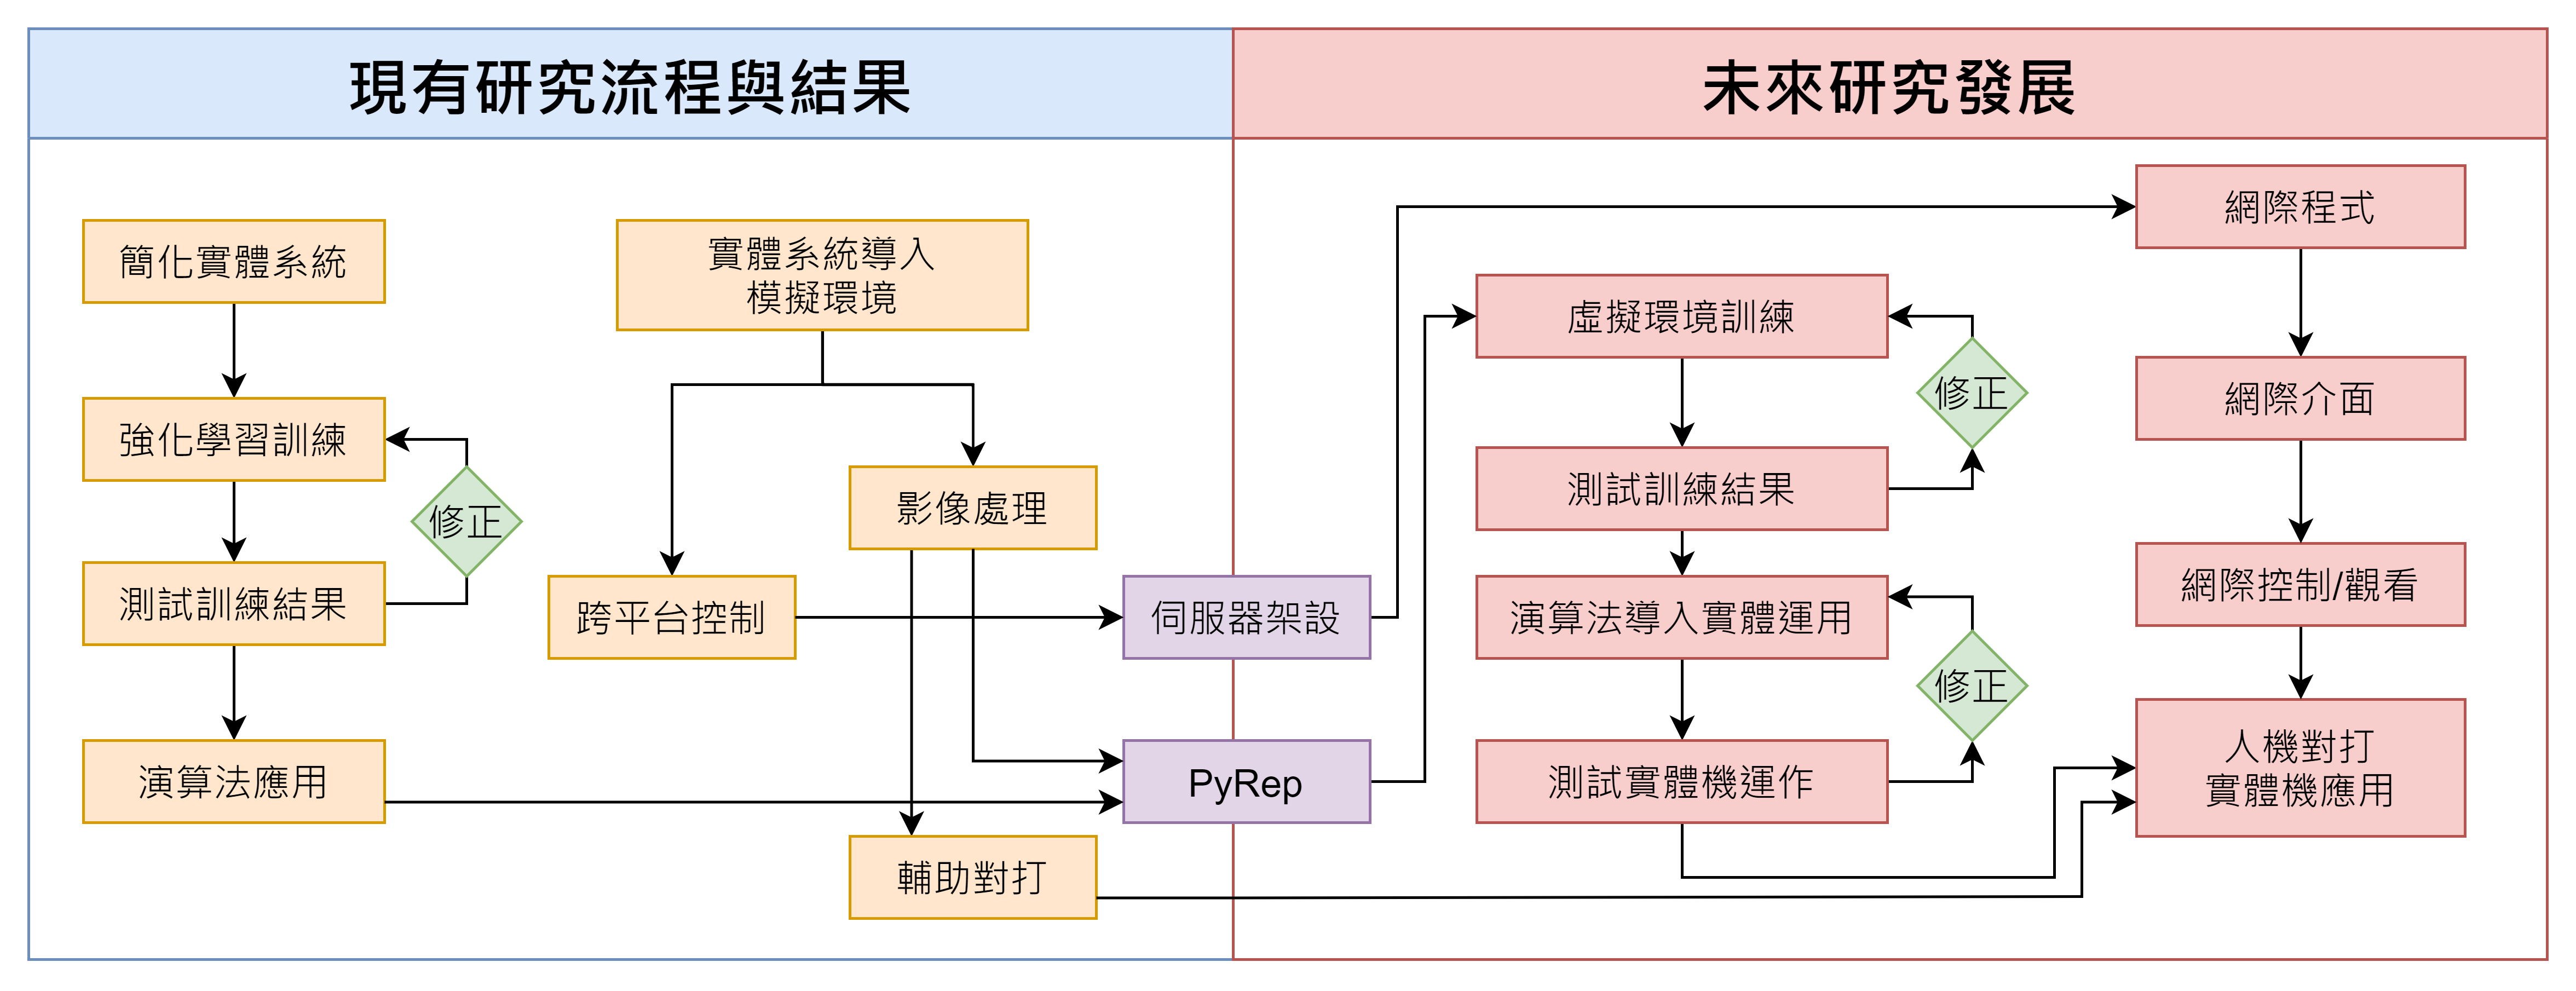
\includegraphics[width=16cm]{現有研究流程與未來展望}
\caption{\Large 現有研究流程與未來展望}
\label{fig.現有研究流程與未來展望}
\end{center}
\end{figure}

\chapter{問題與討論}
\hspace{-1.7em} Q:gym用到的atari動態連結庫在讀取目錄下但在執行的時候出現缺少 ale\_ c.cp38-win\_ amd64.dll\\
\begin{figure}[hbt!]
\begin{center}
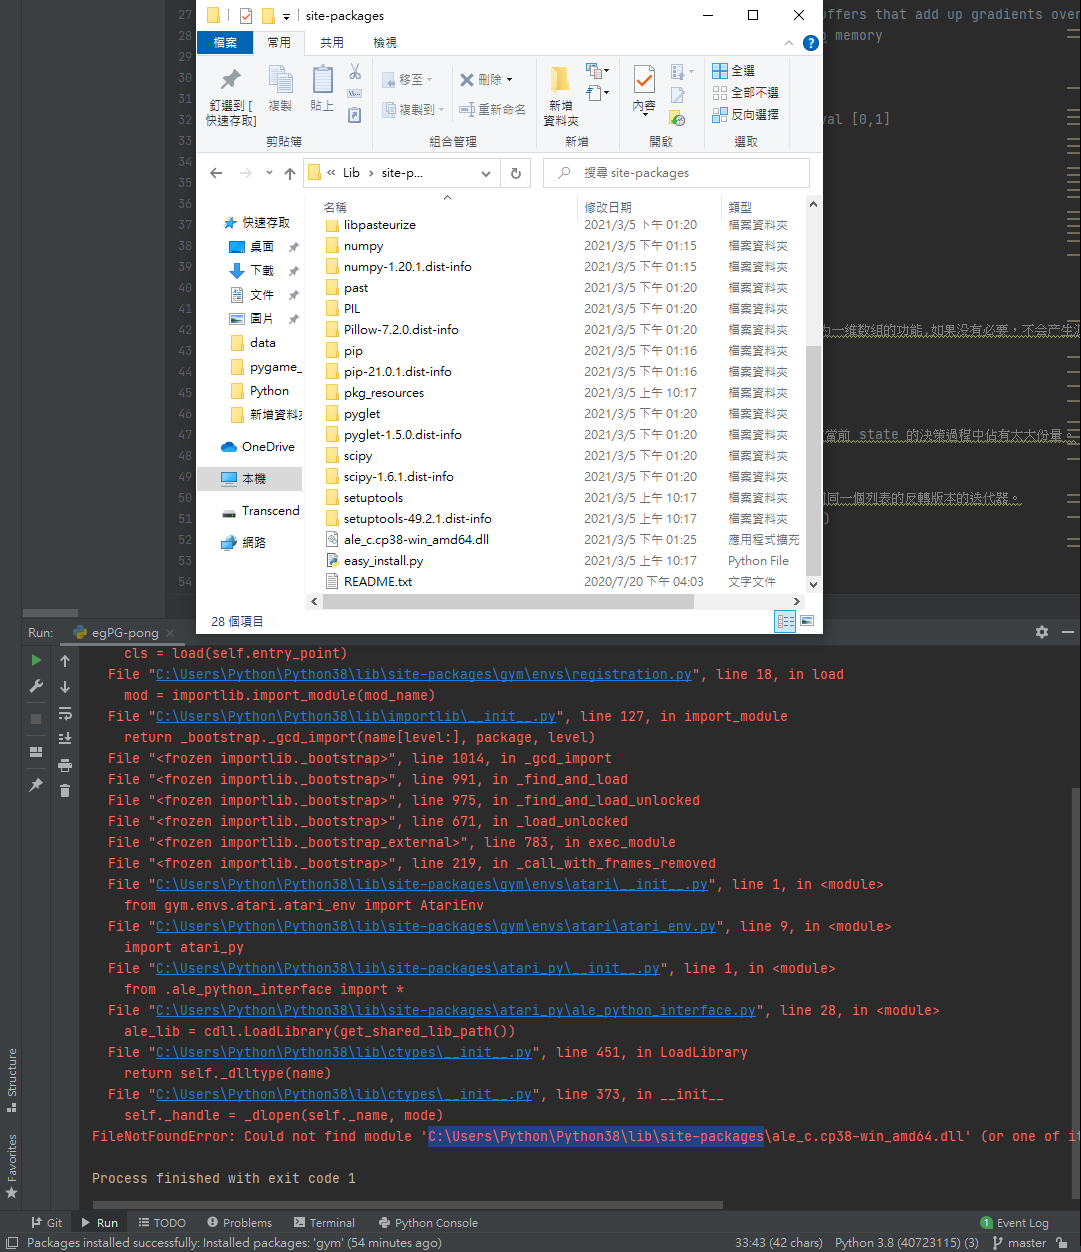
\includegraphics[width=15cm]{Q_dll}
\caption{\Large 動態連結庫錯誤}
\label{fig.動態連結庫錯誤}
\end{center}
\end{figure}
\newpage
\hspace{-1.4em}A:此問題尚未找到解決方法。\\
Q:錄製訓練過程的程式讀不到ffmpeg(圖.\ref{fig.Q_ffmpeg})。\\
\begin{figure}[hbt!]
\begin{center}
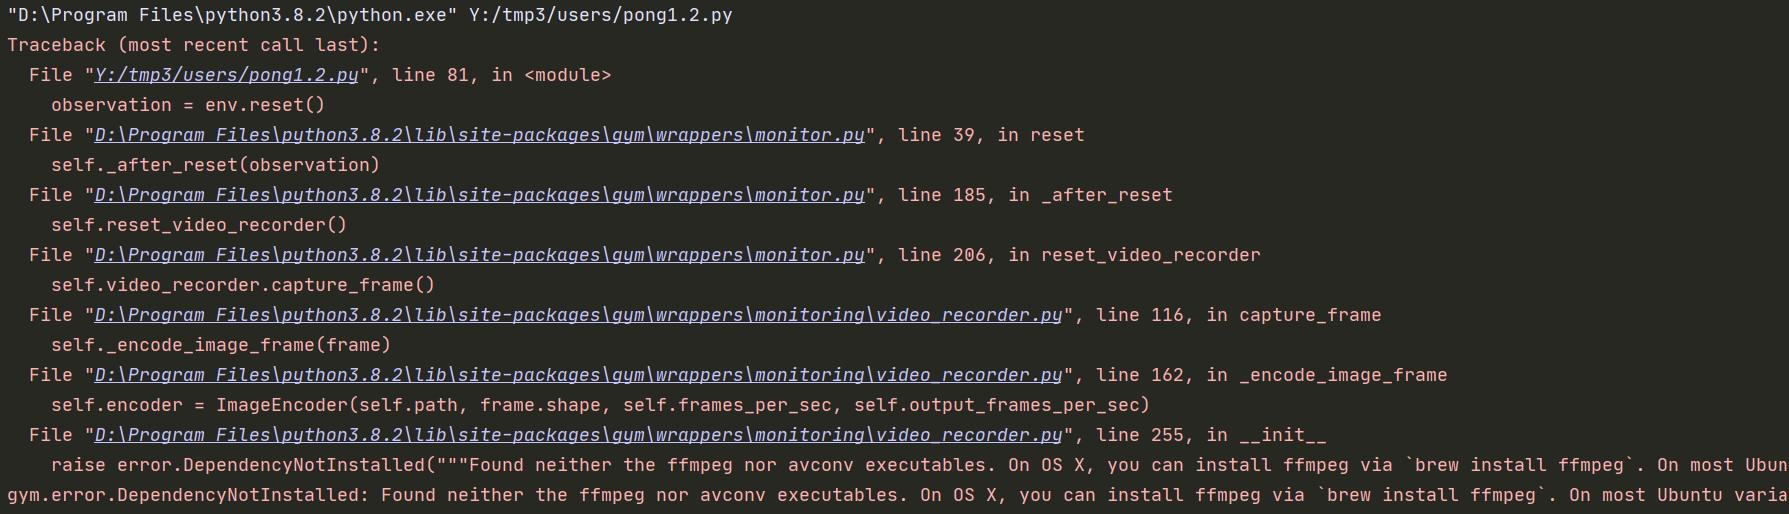
\includegraphics[width=15cm]{Q_ffmpeg}
\caption{\Large 程式讀不到ffmpeg}
\label{fig.Q_ffmpeg}
\end{center}
\end{figure}
\qquad \\
A:需要在作業系統中安裝ffmpeg:
\begin{enumerate}
\item 下載、解壓縮\\
先到官網 \href{https://ffmpeg.org/download.html}{https://ffmpeg.org/download.html} 下載" \href{https://www.gyan.dev/ffmpeg/builds/}{Windows builds from gyan.dev} ",下載 \href{https://www.gyan.dev/ffmpeg/builds/ffmpeg-git-full.7z}{https://www.gyan.dev/ffmpeg/builds/ffmpeg-git-full.7z} ,解壓縮重新命名成"ffmpeg"並放到C槽目錄下(C:$\setminus$ffmpeg)。
\item 環境設定(windows10 20H2 及 2004版本)\\
開啟"設定"→"系統"→左方"關於"選項→右側"進階系統設定"→"環境變數"(圖.\ref{fig.Q_ffmpeg-2})→選取"Path",編輯(圖.\ref{fig.Q_ffmpeg-3})→"新增",增加一個環境變數,給定內容為:"C:$\setminus$ffmpeg$\setminus$bin","確定"(圖.\ref{fig.Q_ffmpeg-4})→"確定"→"確定\\
\end{enumerate}
\begin{figure}[hbt!]
\begin{center}
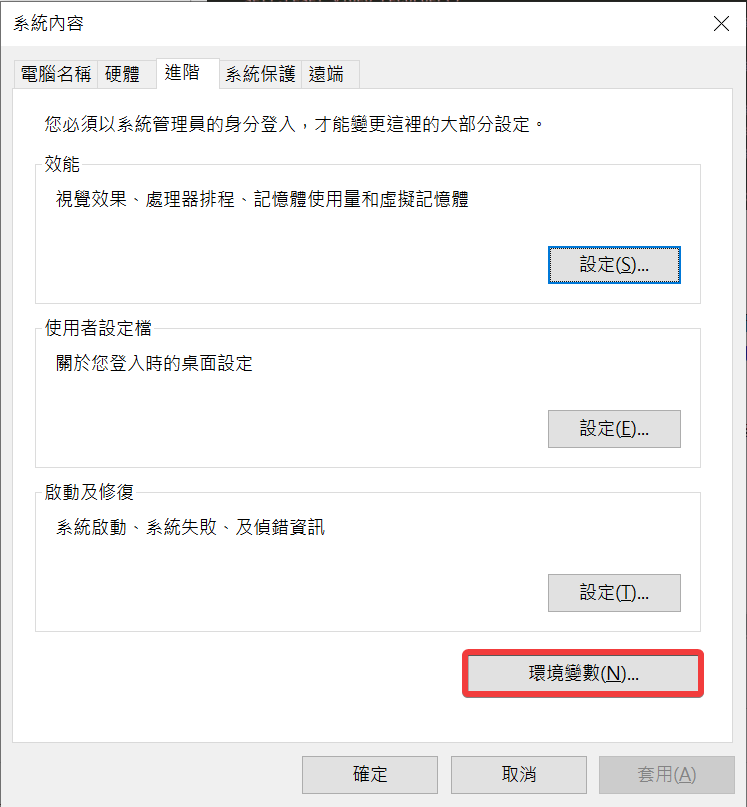
\includegraphics[width=10cm]{Q_ffmpeg-2}
\caption{\Large 進階系統設定}
\label{fig.Q_ffmpeg-2}
\end{center}
\end{figure}
\fontsize{0.001pt}{1pt}\selectfont .\\ %圖片間距勿刪
\begin{figure}[hbt!]
\begin{center}
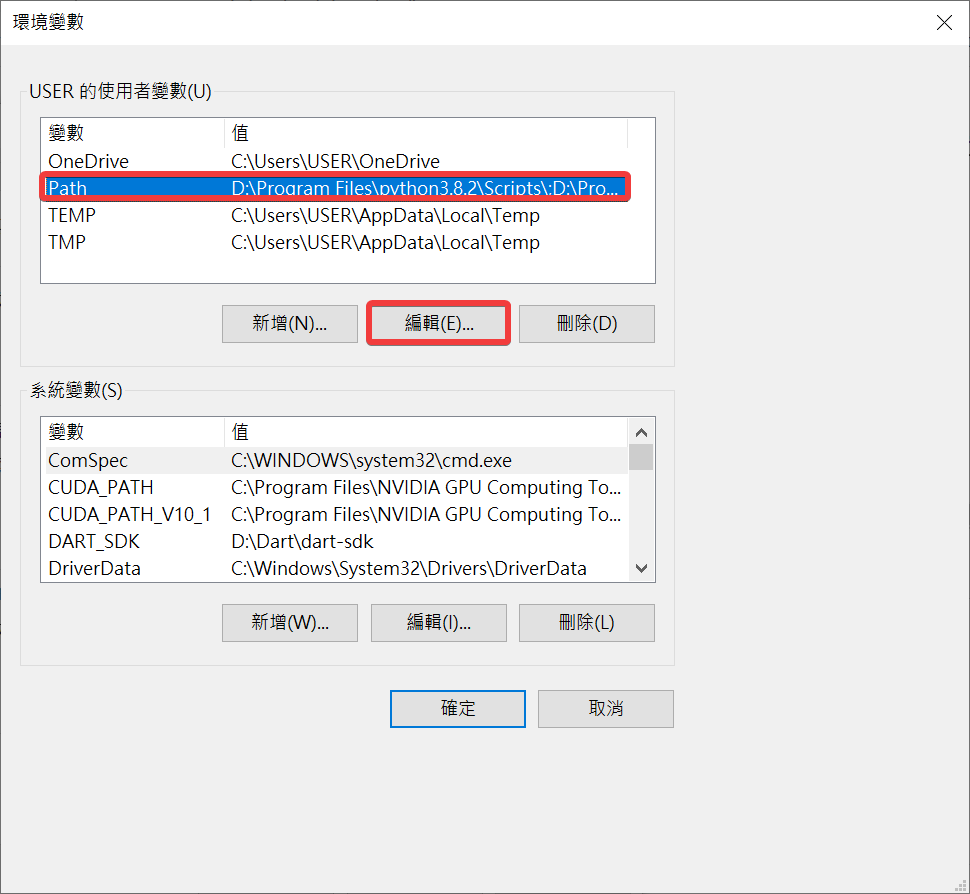
\includegraphics[width=10cm]{Q_ffmpeg-3}
\caption{\Large 環境變數}
\label{fig.Q_ffmpeg-3}
\end{center}
\end{figure}
\fontsize{0.001pt}{1pt}\selectfont .\\ %圖片間距勿刪
\newpage
\begin{figure}[hbt!]
\begin{center}
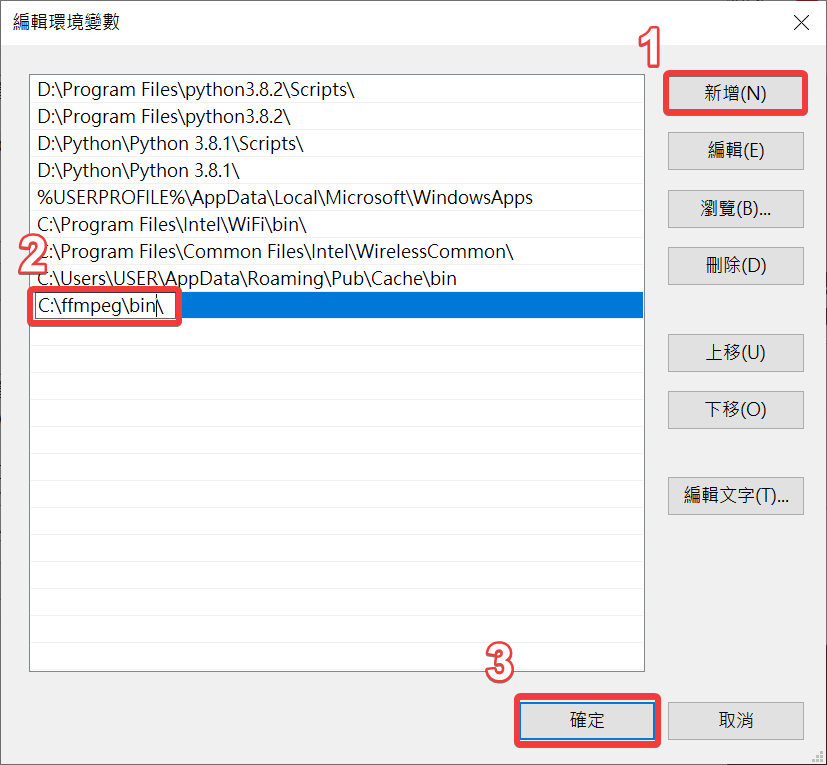
\includegraphics[width=15cm]{Q_ffmpeg-4}
\caption{\Large 編輯環境變數}
\label{fig.Q_ffmpeg-4}
\end{center}
\end{figure}
\fontsize{0.001pt}{1pt}\selectfont .\\ %圖片間距勿刪

\newpage %圖片間距勿刪
\fontsize{14pt}{28pt}\selectfont

\begin{itemize}
\item 測試\\
開啟命令字元(win+R,輸入"cmd"),執行"ffmpeg"(圖.\ref{fig.Q_ffmpeg-5})\\

\begin{figure}[hbt!]
\begin{center}
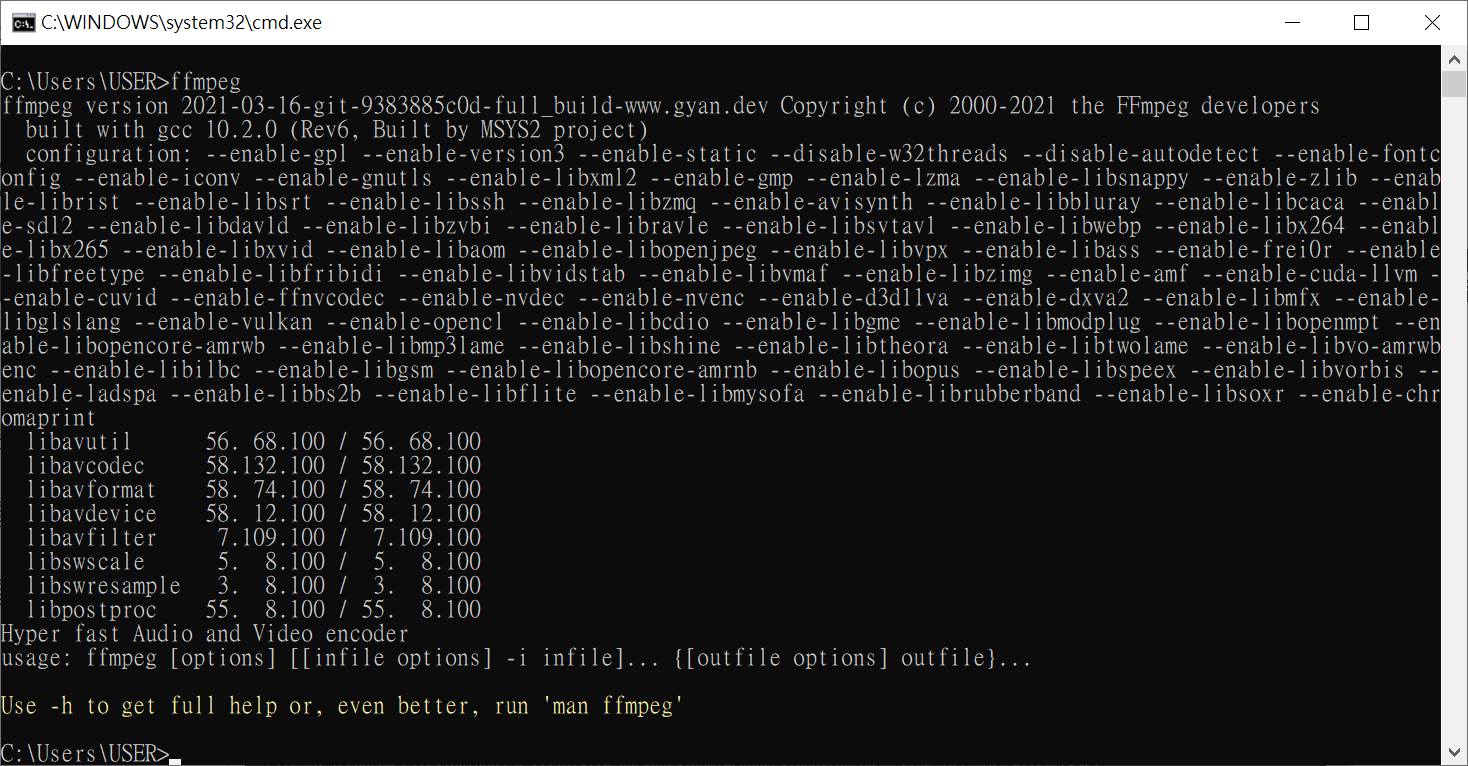
\includegraphics[width=15cm]{Q_ffmpeg-5}
\caption{\Large ffmpeg成功執行}
\label{fig.Q_ffmpeg-5}
\end{center}
\end{figure}
\end{itemize}
\newpage%圖片間距勿刪
\hspace{-1.7em} Q:運用gym.wrappers.Monitor透過ffmpeg進行錄影,紀錄下訓練影像。但記錄後的影像資料皆為1KB,並且無法開啟。(圖.\ref{fig.ffmpeg_mp4})\\
\begin{figure}[hbt!]
\begin{center}
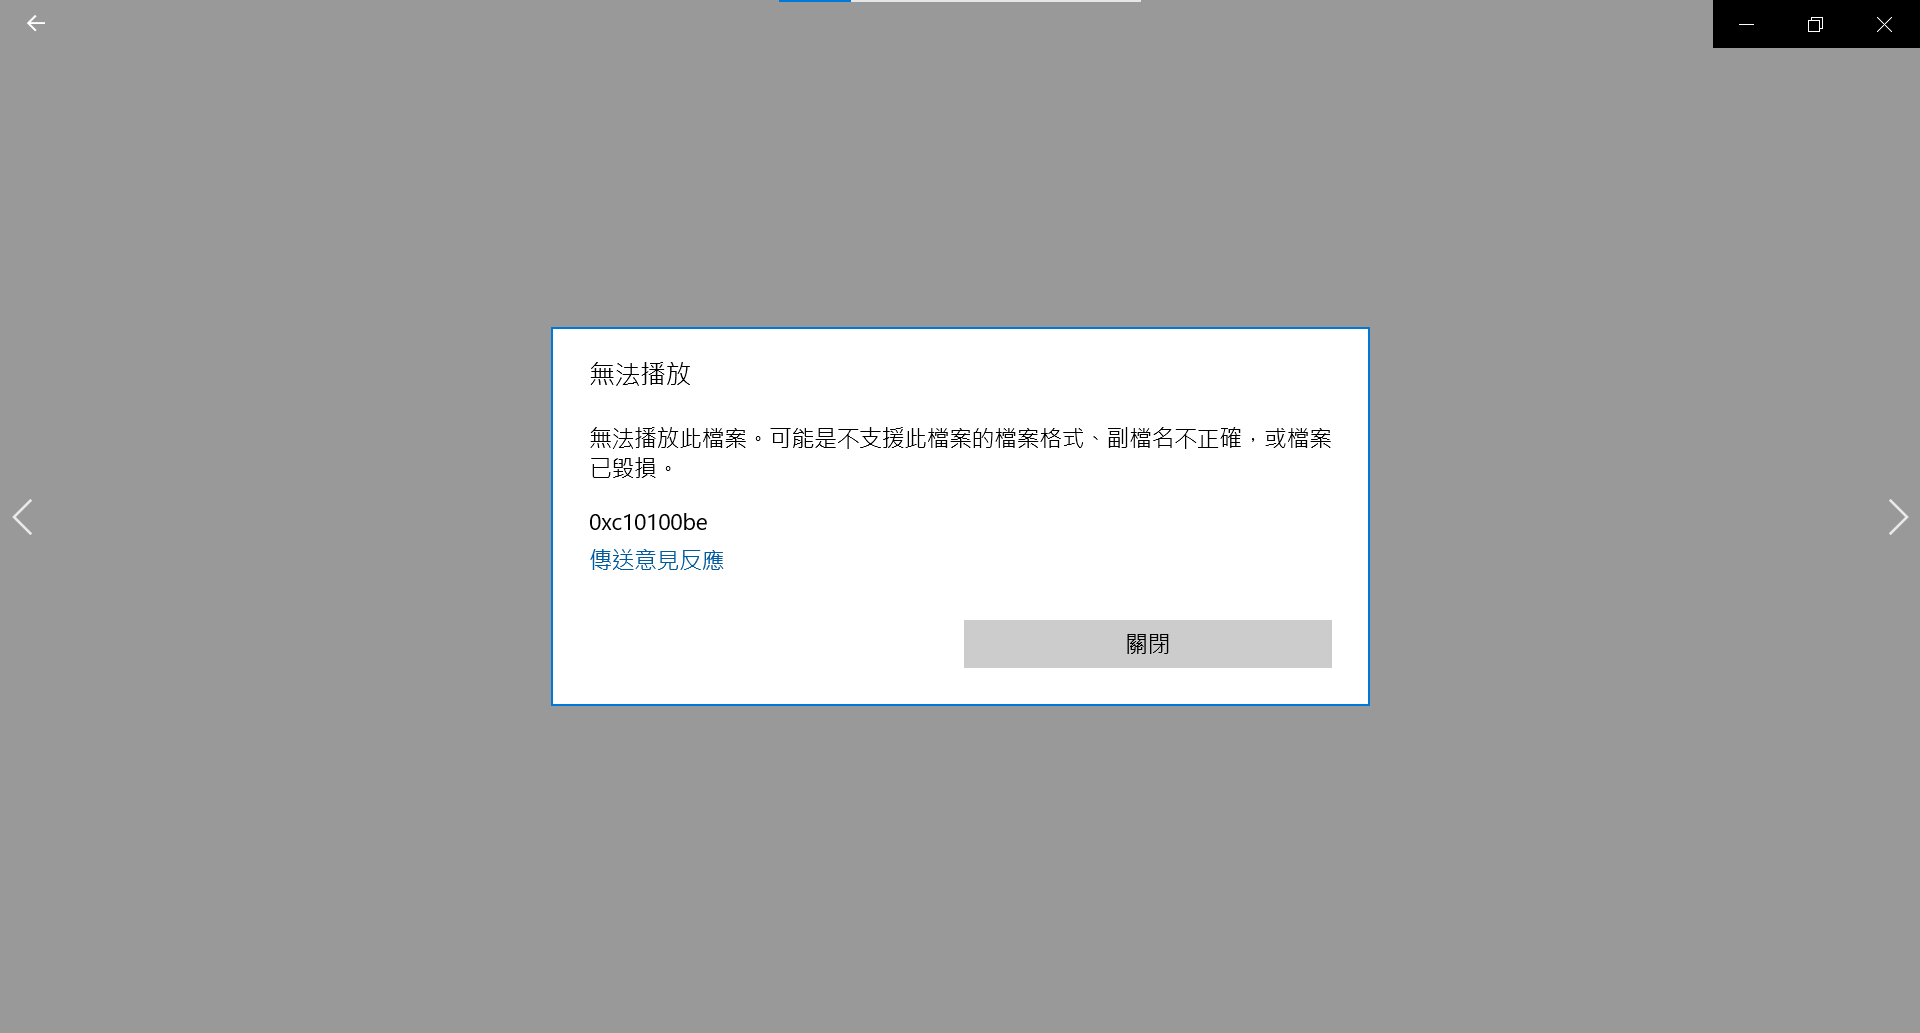
\includegraphics[width=15cm]{ffmpeg_mp4}
\caption{\Large 錄製後,影片無法開啟}
\label{fig.ffmpeg_mp4}
\end{center}
\end{figure}
\qquad \\%圖片間距勿刪
%圖片間距勿刪
A:修改g ym.wrappers.Monitor的video\_ recorder.py的設定(圖.\ref{fig.video_recorder}),將303行的縮排修正(從if階層上移到def的階層)即可(圖.)。\\
\begin{figure}[hbt!]
\begin{center}
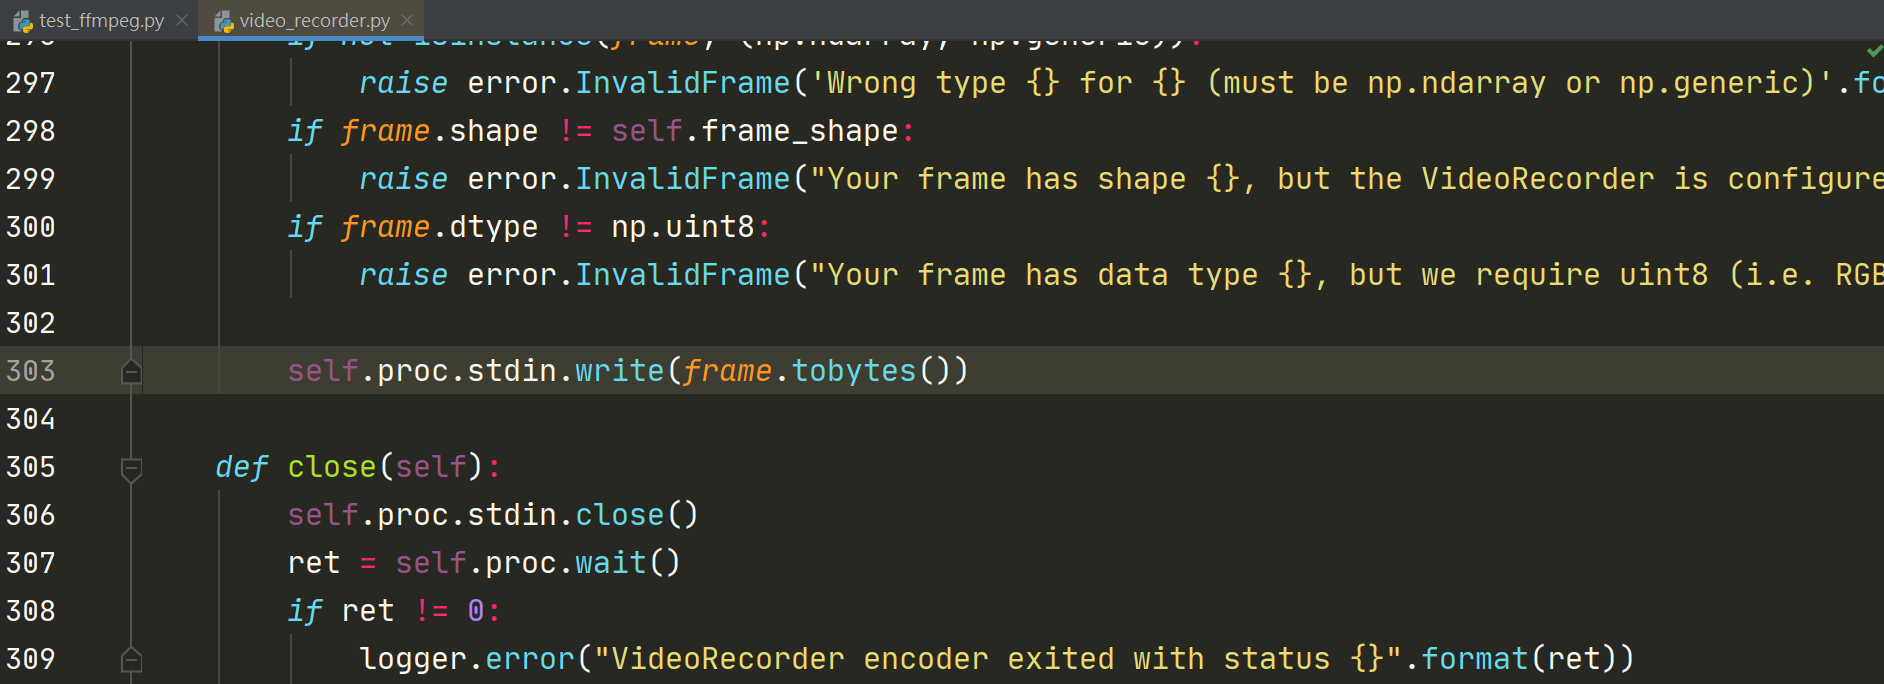
\includegraphics[width=15cm]{video_recorder}
\caption{\Large 原始設定}
\label{fig.video_recorder}
\end{center}
\end{figure}

\begin{figure}[hbt!]
\begin{center}
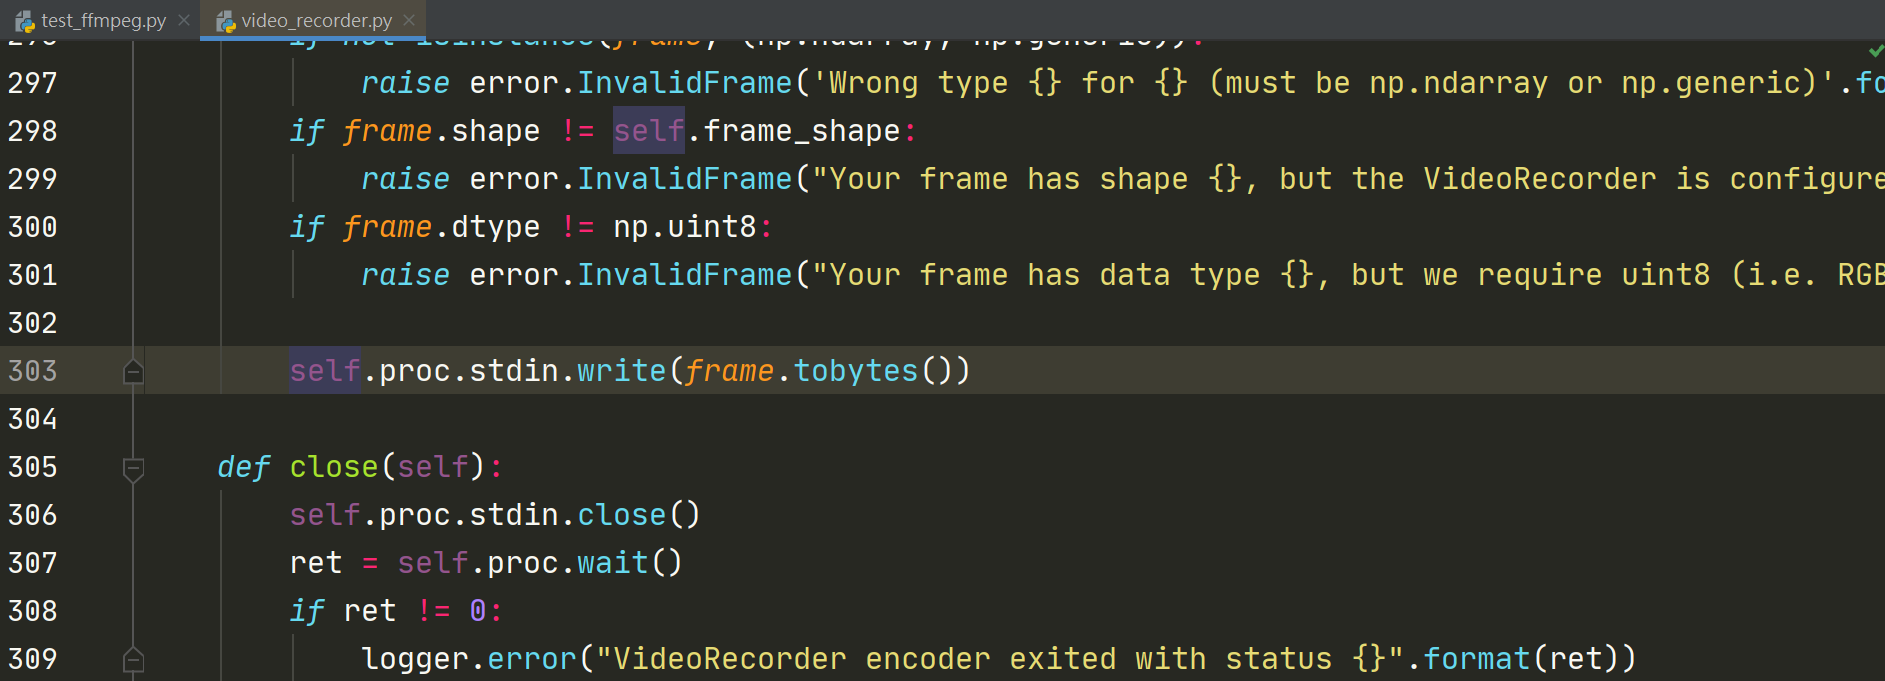
\includegraphics[width=15cm]{修正video_recorder}
\caption{\Large 修正後設定}
\label{fig.修正video_recorder}
\end{center}
\end{figure}
\newpage %圖片間距勿刪

\hspace{-1.7em} Q:啟用cmsimde的MathJax的功能遇到文章使用括號補充說明的內容被誤當成latex的語法轉換。\\
\hspace{-1.7em} A:格式轉換原始定義成"("和")",所以出現誤換的問題。\\
\begin{lstlisting}[caption=\Large\sectionef MathJax 程式碼]
<script>
  MathJax = {
    tex: {inlineMath: [['$', '$'], ['\\(', '\\)']]}
  };
  </script>
  <script id="MathJax-script" 
  async src="https://cdn.jsdelivr.net/npm/mathjax@3/es5/tex-chtml.js"> 
  </script>
\end{lstlisting}

修正後將"("和")"換成"\$",就解決誤換問題
%=---------------------參考文獻----------------------=%
\addcontentsline{toc}{chapter}{參考文獻} %新增目錄名稱
\newpage
\renewcommand\bibname{參~考~文~獻}
\begin{thebibliography}{99}  % 參考文獻印出之編號最寬為兩個字母寬
\bibitem 1\href{https://towardsdatascience.com/adam-latest-trends-in-deep-learning-optimization-6be9a291375c}{https://towardsdatascience.com/adam-latest-trends-in-deep-learning-optimization-6be9a291375c}
\bibitem 2\href{https://towardsdatascience.com/derivative-of-the-sigmoid-function-536880cf918e}{https://towardsdatascience.com/derivative-of-the-sigmoid-function-536880cf918e}
\bibitem 3\href{http://www.incompleteideas.net/book/RLbook2020.pdf}{http://www.incompleteideas.net/book/RLbook2020.pdf}
\bibitem 4\href{https://medium.com/change-the-world-with-technology/policy-gradient-181d43a24cf5}{https://medium.com/change-the-world-with-technology/policy-gradient-181d43a24cf5}
\bibitem 5\href{https://livebook.manning.com/book/grokking-deep-reinforcement-learning/chapter-11/v-11/38}{https://livebook.manning.com/book/grokking-deep-reinforcement-learning/chapter-11/v-11/38}
\bibitem 6\href{http://ukko.life.nctu.edu.tw/~u0517047/usage.html}{http://ukko.life.nctu.edu.tw/~u0517047/usage.html}
\bibitem 7\href{https://lilianweng.github.io/lil-log/2018/04/08/policy-gradient-algorithms.html}{https://lilianweng.github.io/lil-log/2018/04/08/policy-gradient-algorithms.html}\label{R.Policy Gradient}
\bibitem 8\href{https://uupgrade.medium.com/python-那些年我們一起玩過的遊戲-三-打磚塊-d89b648896ca}{https://uupgrade.medium.com/python-那些年我們一起玩過的遊戲-三-打磚塊-d89b648896ca}
\bibitem 9\href{https://cvfiasd.pixnet.net/blog/post/275774124-深度學習激勵函數介紹}{https://cvfiasd.pixnet.net/blog/post/275774124-深度學習激勵函數介紹}
\bibitem 0\href{https://www.coppeliarobotics.com/helpFiles/}{https://www.coppeliarobotics.com/helpFiles/}
\bibitem 1\href{https://hackernoon.com/the-reason-behind-moving-in-the-direction-opposite-to-the-gradient-f9566b95370b}{https://hackernoon.com/the-reason-behind-moving-in-the-direction-opposite-to-the-gradient-f9566b95370b}\label{OGD}
\bibitem 2\href{https://ruder.io/optimizing-gradient-descent/}{https://ruder.io/optimizing-gradient-descent/}
\label{OGD2}
\bibitem 3\href{https://reurl.cc/43XjEL}{https://zh.wikipedia.org/wiki/HSL和HSV色彩空間}
\label{RGBtoHSV}
\bibitem 4\href{https://reurl.cc/gzMm4N}{https://gist.github.com/karpathy/a4166c7fe253700972fcbc77e4ea32c5\# file-pg-pong-py}\label{R.pong1}
\bibitem 5\href{https://reurl.cc/95172Y}{https://github.com/schinger/pong\_ actor-critic/blob/master/pg-pong-ac.py}\label{R.pong1.1}
\bibitem 6\href{https://gist.github.com/etienne87/6803a65653975114e6c6f08bb25e1522}{https://gist.github.com/etienne87/6803a65653975114e6c6f08bb25e1522}\label{R.pong2}
%\bibitem 7\href
%\bibitem 8\href
%
%\bibitem 3\href{https://blog.csdn.net/Csdn_Darry/article/details/107142216}{https://blog.csdn.net/CsdnDarry/article/details/107142216}
\end{thebibliography}
\newpage
%=---------------附錄-----------------=%
\addcontentsline{toc}{chapter}{附錄} %新增目錄名稱
\begin{appendix}
\renewcommand{\thesection}{\bf 附錄 \Alph{section}}%設定標題名稱
\begin{center}
\fontsize{20pt}{0em}\selectfont\bf 附錄
\end{center}
\section*{LaTeX}
LaTex 為一種程式語言,支援標準庫 (Standard Libraries) 和外部程式庫 (External Libraries),不過與一般程式語言不同的是,它可以直接表述 Tex 排版結構,類似於 PHP 之於 HTML 的概念。但是直接撰寫 LaTex 仍較複雜,因此可以藉由 Markdown 這種輕量的標註式語言先行完成文章,再交由 LaTex 排版。
此專題報告採用編輯軟體為LaTeX,綜合對比Word編輯方法,LaTeX較為精準正確、更改、製作公式等,以便符合規範、製作。
 \begin{table}[htbp] %htbp代表表格浮動位置
			\centering%表格居中
			\caption{文字編輯軟體比較表}%表:標題
			\large%字體大小
			\label{tab_文字編輯軟體比較表:scale}
			\begin{tabular}{|c|c|c|c|c|c|c|}
			\hline
			\diagbox[width=5em]& 相容性 & 直觀性 & 文件排版 & 數學公式 & 微調細部\\ 
			\hline
			LaTeX 		&$\surd$&		&$\surd$&$\surd$&$\surd$\\
			\hline
			Word	 	&		&$\surd$&		&		&$\surd$\\
			\hline
			
			\end{tabular}
		\end{table}	

\begin{itemize} 
\item 特點:
\end{itemize}
\begin{enumerate}
\item 相容性:以Word為例會有版本差異,使用較高版本編輯的文件可能無法以較低的版本開啟,且不同作業系統也有些許差異;相比LaTeX可以利用不同編譯器進行編譯,且為免費軟體也可移植至可攜系統內,可以搭配Github協同編譯。
\item 文件排版:許多規範都會要求使用特定版型,使用文字編譯環境較能準確符合規定之版型,且能夠大範圍的自定義排定所需格式,並能不受之後更改而整體格式變形。
\item 數學公式呈現:LaTex可以直接利用本身多元的模組套件加入、編輯數學公式,在數學推導過程能夠快速的輸入自己需要的內容即可。
\item 細部調整:在大型論文、報告中有多項文字、圖片、表格,需要調整細部時,要在好幾頁中找尋,而LaTeX可以分段章節進行編譯,再進行合併處理大章節。
\end{enumerate}
\begin{figure}[hbt!]
\begin{center}
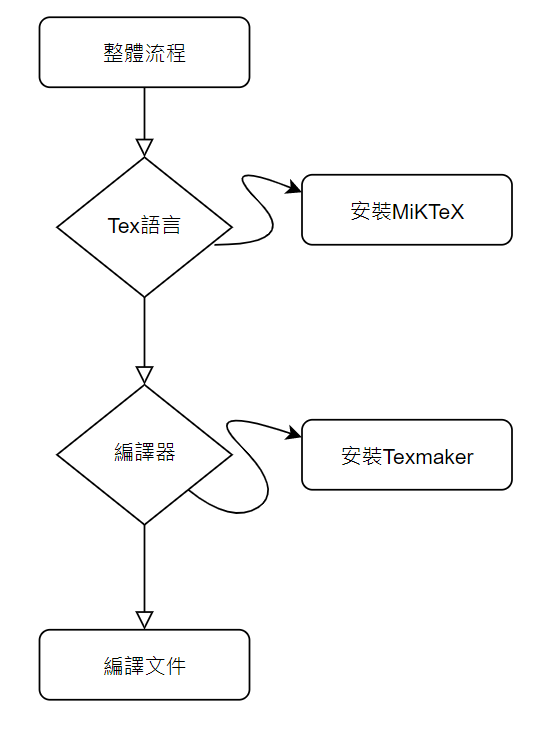
\includegraphics[width=10cm]{編譯流程}
\caption{\Large 編譯流程}
\label{fig.編譯流程}
\end{center}
\end{figure}
\end{appendix}
\section*{FFmpeg}
FFmpeg是一個開放原始碼的自由軟體,可以對音訊和視訊進行多種格式的錄影、轉檔、串流功能。在專題訓練過程中透過FFmpeg的視訊錄製的功能記錄對打影像來了解實際訓練狀況。
\newpage
\newpage
%=-------------作者簡介-----------------=%
 
%=----------------書背----------------------=%

